\documentclass[onecolumn, draftclsnofoot,10pt, compsoc]{IEEEtran}
\usepackage{graphicx}
\graphicspath{{./images/}}

\usepackage{url}
\usepackage{setspace}
\usepackage{csquotes}
\usepackage{float}
\usepackage{soul}
\usepackage{color}
\usepackage{pstricks-add}
\usepackage{hyperref}

\usepackage{listings}
\RequirePackage{pgfcalendar}
\usepackage{pgfgantt}
\usepackage{pdflscape}
\usepackage{tikz}

% COLOR DEFINITIONS FOR CODE LISTINGS
\definecolor{codegreen}{rgb}{0,0.6,0}
\definecolor{codegray}{rgb}{0.5,0.5,0.5}
\definecolor{codepurple}{rgb}{0.58,0,0.82}
\definecolor{backcolour}{rgb}{0.95,0.95,0.92}

\lstdefinestyle{mystyle}{
    backgroundcolor=\color{backcolour},
    commentstyle=\color{codegreen},
    keywordstyle=\color{magenta},
    numberstyle=\tiny\color{codegray},
    stringstyle=\color{codepurple},
    basicstyle=\footnotesize,
    breakatwhitespace=false,
    breaklines=true,
    captionpos=b,
    keepspaces=true,
    numbers=left,
    numbersep=5pt,
    showspaces=false,
    showstringspaces=false,
    showtabs=false,
    tabsize=2
}

\lstset{
	escapeinside={(*@}{@*)},
	style=mystyle
}

\usepackage{geometry}
\geometry{textheight=9.5in, textwidth=7in}

% 1. Fill in these details
\def \CapstoneTeamName{	Short Circuit Comedy Club	}
\def \CapstoneTeamNumber{		CS13}
\def \GroupMemberOne{			Kevin Talik}
\def \GroupMemberTwo{			Arthur Shing}
\def \GroupMemberThree{			Anish Asrani}
\def \CapstoneProjectName{		How to Build an Effective Robot Comedian}
\def \CapstoneSponsorCompany{	Oregon State University}
\def \CapstoneSponsorPerson{		Dr. Heather Knight}

% 2. Uncomment the appropriate line below so that the document type works
\def \DocType{		%Problem Statement
				%Requirements Document
				%Technology Review
				%Design Document
				Final Document
				}

\newcommand{\NameSigPair}[1]{\par
\makebox[2.75in][r]{#1} \hfil 	\makebox[3.25in]{\makebox[2.25in]{\hrulefill} \hfill		\makebox[.75in]{\hrulefill}}
\par\vspace{-12pt} \textit{\tiny\noindent
\makebox[2.75in]{} \hfil		\makebox[3.25in]{\makebox[2.25in][r]{Signature} \hfill	\makebox[.75in][r]{Date}}}}
% 3. If the document is not to be signed, uncomment the RENEWcommand below
%\renewcommand{\NameSigPair}[1]{#1}

%%%%%%%%%%%%%%%%%%%%%%%%%%%%%%%%%%%%%%%
\begin{document}
\begin{titlepage}
    \pagenumbering{gobble}
    \begin{singlespace}
 %   	\includegraphics[height=4cm]{coe_v_spot1}
        \hfill
        % 4. If you have a logo, use this includegraphics command to put it on the coversheet.
        %\includegraphics[height=4cm]{CompanyLogo}
        \par\vspace{.2in}
        \centering
        \scshape{
            \huge CS Capstone \DocType \par
            {\large\today}\par
            \vspace{.5in}
            \textbf{\Huge\CapstoneProjectName}\par
            \vfill
            {\large Prepared for}\par
            \Huge \CapstoneSponsorCompany\par
            \vspace{5pt}
            {\large Prepared by }\par
            Group\CapstoneTeamNumber\par
            % 5. comment out the line below this one if you do not wish to name your team
            \CapstoneTeamName\par
            \vspace{5pt}
            \vspace{20pt}
        }
        \begin{abstract}
  	     % 6. Fill in your abstract
			The purpose of this document is to outline the research papers that this team will create to conclude during Spring Term 2018.
			The three members of the \textit{Short Circut Comedy Club} have spent their time during winter term perfomring research under Dr. Heather Knight at Oregon State University.
			The focus of this project is to study the effect a robot comedian can have on a crowd of humans.
			Kevin Talik's research has been spent understanding what a Comedian can do to "Adapt" to a performance.
			Arthur Shing has been studying the voice of the robot, and the difference between "Robot and Human" character.
			One final aspect of Stand-Up Comedy that we studied is "Crowd Work". Anish Asrani has spent most of his time developing spontaneous Crowd-Interactions during the set.
        \end{abstract}
    \end{singlespace}
\end{titlepage}
\newpage
\pagenumbering{arabic}
\tableofcontents
% 7. uncomment this (if applicable). Consider adding a page break.
%\listoffigures
%\listoftables
\clearpage


\section{Introduction to Project}
This project was requested by Dr. Heather Knight, a Computer Science professor at Oregon State University.
Dr. Knight purposed this project to be a pilot research project, to investigate how aspects of comedy can improve a robot's charisma in Human-Robot Interaction (HRI).


This project, if successful, can benefit and influence the fields of comedy and HRI by showing how certain features of a robot comedian can be conducive to creating an entertaining encounter between a human and a comedian or robot.

In stand-up comedy, comedians have to rely on their scripted jokes and their ability to improvise to have a successful performance. In many ways, a robot interaction can be compared to a stand-up set. Within the context of stand up comedy, a robot must be receptive to an audience and tell jokes to make an audience laugh.

Why is the field of robot comedy relevant and worth studying? With automation slowly replacing menial tasks in society, such as an ATM or an automated cashier, interactions with bots are going to be much more common. These machines are less engaging to interact with, but require reciprocity to obtain a goal. While these machines do improve ease of use and convenience, people are not as expressive towards the robot. Even if the machine is unsuccessful in completing its task, expressive robots are received in a more empathetic manner by the users {\cite{DesignExBeh:2017}}. The user’s perception of a robot’s expression is more significant than its true internal state when seeking to generate engaging interactions {\cite{KnightEightLessons:2011}}.

Dr. Heather Knight noted the importance of the audience recognizing the performer as a social being, rather than as a dull object. In this respect, artificial social intelligence can bring greater engagement to the realm of the theatre. A socially intelligent robot comedian can be crafted by utilizing non-verbal gestures and by conveying a sense of character through spontaneous interactions with the audience {\cite{KnightEightLessons:2011}}.  Additionally, a study by Katevas et al. {\cite{RobotComedyLab:2015}} evaluated the influence of non-verbal aspects of joke delivery. Knight also noted how physical presence and embodiment in a robot creates a more expressive and engaging interaction {\cite{KnightEightLessons:2011}}. In another study done by Sjöbergh and Araki {\cite{RobotsMakeThings:2008}}, having a robot tell a joke was found to generate more of an audience reaction than having the joke read by a human. However, this study evaluated joke performance by a robot, but not an entire stand-up set. To extend on these lines of research, we intend to focus on the effect of verbally and physically expressing robot character qualities during a stand-up performance.

\subsection{Team Members}
The members of our team are Kevin Talik, Anish Asrani, and Arthur Shing. Kevin acted as team leader, and focused on creating the adaptive portion of the robot comedian. Anish focused on creating the audience sensing and crowdwork portion of the robot comedian. Arthur focused on creating topical variations of robot and human versions of jokes, as well as animations for the robot comedian. Our client, Dr. Heather Knight, supervised and worked along with us in many parts of the project. She often provided guidance or help in areas of development that we had trouble with.  

\pagebreak

\input{reqdoc.tex}


\subsection{Modified Requirements}
In terms of modified requirements, some of our existing requirements were deleted because they were infeasible to complete in time.
Requirements that were changed include the coherent vs. incoherent character research area. This was modified slowly into the robot vs. human research area, as it was too hard to create an entertaining comedy set with an incoherent comedian. In addition, it became clear at some point in the project that doing multiple official tests would be infeasible, so we decided to do all our tests unofficially at the Engineering Expo.


\pagebreak
\begin{landscape}
	\section{Final Gantt Chart}

	\ganttset{calendar week text = \small{{\startday}}}
	% \resizebox{0}{0}{

	\begin{figure}[H]
		\scalebox{0.82}{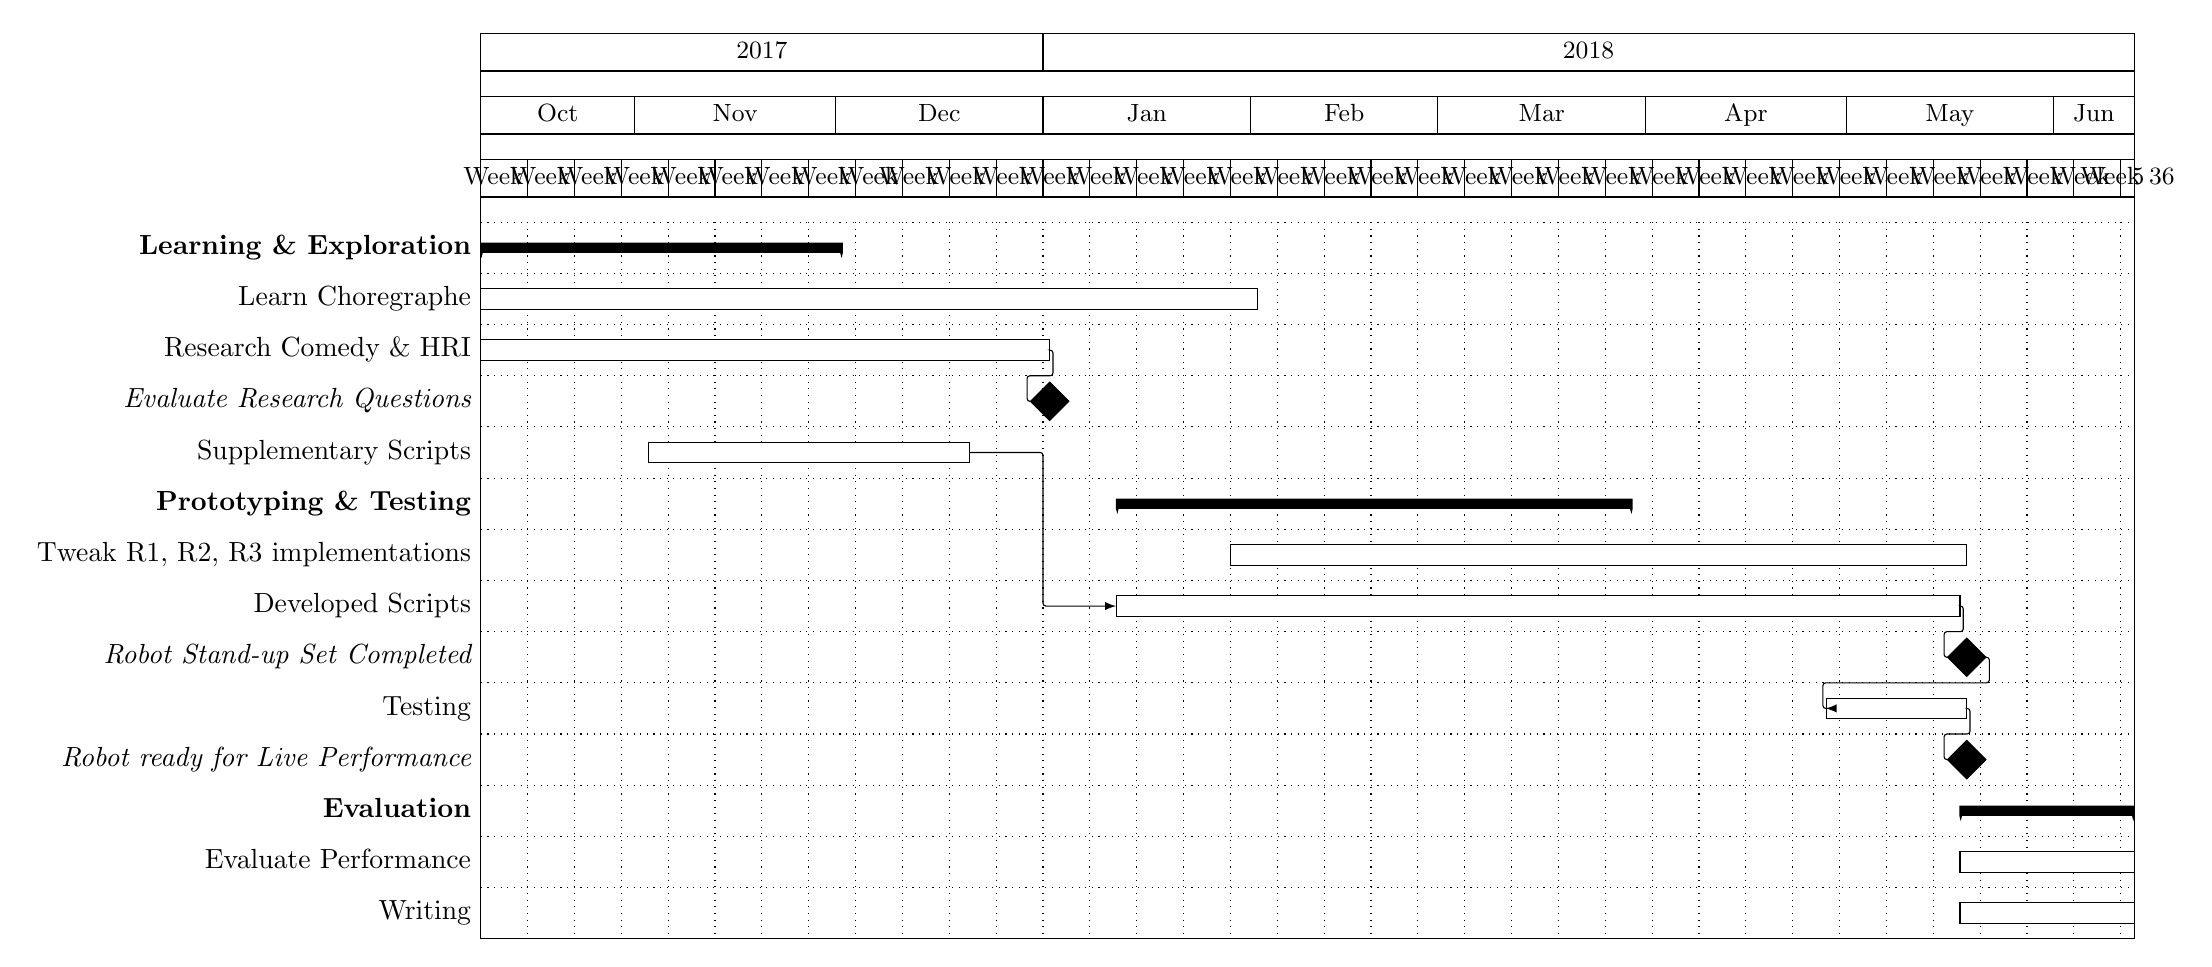
\begin{tikzpicture}[]
\begin{ganttchart}[
	hgrid,
	vgrid={*6{draw=none, dotted}, dotted},
	x unit = 0.085cm,
	y unit title = 0.8cm,
	y unit chart = 0.65cm,
	time slot format=isodate,
	milestone/.append style = {inner sep=3.5pt}
	]{2017-10-09}{2018-06-12}

	\gantttitlecalendar{year, month=shortname, week}{week} \\
	% \gantttitle{Fall}{10}
	% \gantttitle{Winter}{10}
	% \gantttitle{Spring}{7} \\
	\ganttgroup{Learning \& Exploration}{2017-10-09}{2017-12-01} \\
	\ganttbar{Learn Choregraphe}{2017-10-09}{2018-02-01} \\
	\ganttbar[name=Research]{Research Comedy \& HRI}{2017-10-09}{2018-01-01} \\
	\ganttmilestone[name=M1]{Evaluate Research Questions}{2018-01-01} \\
  \ganttbar[name=S1]{Supplementary Scripts}{2017-11-03}{2017-12-20} \\
	\ganttgroup{Prototyping \& Testing}{2018-01-12}{2018-03-29} \\
  \ganttbar[name=Q]{Tweak R1, R2, R3 implementations}{2018-01-29}{2018-05-18} \\
	\ganttbar[name=S2]{Developed Scripts}{2018-01-12}{2018-05-17} \\
  \ganttmilestone[name=M2]{Robot Stand-up Set Completed}{2018-05-18} \\
  \ganttlinkedbar[name=T1]{Testing}{2018-04-28}{2018-05-18} \\
	% \ganttlinkedbar[name=T2]{Video Tests}{16}{20} \\
  \ganttmilestone[name=M3]{Robot ready for Live Performance}{2018-05-18} \\
	\ganttgroup{Evaluation}{2018-05-18}{2018-06-12} \\
	\ganttbar{Evaluate Performance}{2018-05-18}{2018-06-12} \\
	\ganttbar{Writing}{2018-05-18}{2018-06-12}

  \ganttlink{Research}{M1}
	\ganttlink{S1}{S2}
	\ganttlink{S2}{M2}
	\ganttlink{T1}{M3}
	% \ganttlink{M2}{T3}



	% \ganttlink{elem2}{elem3}
	% \ganttlink{elem3}{elem4}
	\end{ganttchart}
\end{tikzpicture}
}
		\caption{A gantt chart showing the timeline of the project.}
		\label{Gantt Chart}
	\end{figure}

\end{landscape}
\pagebreak



\section{Design Document}
\subsection{Introduction}
  Comedy can come from robots of any kind. A carpet cleaning bot could miscalculate the end of a floor and tumble down a flight of stairs, or a voice-assisted tool might accidentally confuse a \textit{Dinnertime Jazz} playlist for \textit{Death Metal Essentials}. These actions that happen around a human can become shared experiences and references for the observer. For every shared task between a robot and a human, the human will often feel more empathetic towards a robot that makes an effort to be more aware of surroundings\cite{DesignExBeh:2017}. If the robot wants to become an effective comedian, it will have to attempt to be empathetic as well; it has to listen to the response of a completed action, and consider the change the bot brought to the setting.

\subsubsection{Scope}
This paper covers the research questions that will guide the investigation of the interaction between a crowd and
a comedian robot, as well as the main design goals for implementing comedy behaviors on a NAO Robot. There
are three areas of intended research. These areas include the development of the intelligent adaptions to the crowd
(”adaptation”), the integration of an audience into the performance of a set (”crowdwork”), and the exploration of
robotic versus human-like storytelling, movement, and reaction to the audience (”character”). All of these components
will culminate into the robot comedian, Ginger. At the end of the academic year, we will have a Robot Comedian that we
have evaluated the effectiveness of. The main end-product is software for the variable stand-up comedy sets performed
by the NAO robot, and the analysis of audience responses to our manipulations in audience adaptation, crowdwork,
and robot or human-like character. Both of these will be described in our final paper.


  \subsubsection{Purpose}
	The purpose of this document is to describe the development of the robot comedian, which involves: (1) the three
main research questions, (2) the robot behavior implementations, and (3) the experiments we plan to use to answer the
research questions.

\subsubsection{Intended Audience}
	This document is intended for stakeholders and developers in the research project \textit{How to Make an Effective Robot Comedian}.

	% The first subsection covers the adaptation algorithm, the components of a stand-up set, and audience response comprehension. The next subsection explains "crowd-work", and how we will examine the influence of incorporating the audience into the robot's performance. Finally, the last subsection will cover the diversity of being a robot comedian, and how the qualities of a robot characterize the comedian.

\subsection{Research Design Overview}
This subsection will cover the research questions for evaluating the effectiveness of a robot comedian. These questions will
be the basis of the implementation of the comedian system. All three research questions will be presented including
software requirements needed to answer the questions, and the experimental methods that will generate quantitative
data about what impacts audience experience, participation, and reactions.
The comedian system that is implemented will test three critical areas of a comedic performance corresponding
to our research. The first question is about \textbf{adaptation} of a performance – how the robot and interpret an audience
response. The second question studies \textbf{crowd work} during a show, and the choices a Comedian can make to engage the
audience. Lastly, the third considers the implications of a perceivable \textbf{character} that the robot can portray, in particular robotic versus human-like.


\subsubsection{Adaptation}
\paragraph{Goal}
We hypothesize that audiences will prefer a robot that acknowledges them, and integrates their data and responses into
its set. To test this hypothesis we propose two tests: (1) to transition to topics dependent on the audience response,
and (2) to present a crowd report upon completion of the set. The goal of this portion of the project is to determine
if incorporating the audience into the set will enhance the overall performance of the comedian. To evaluate these
hypotheses, we will conduct live studies in which people experience different versions of the software described below.
\paragraph{Methods}
Generally, the performance will have two to three parts: the Seed Jokes, the Middle Content, and the Close. The Seed
will influence the Middle Content (which will be chosen themed jokes and basis of the show). The Middle Content will
transition to a intelligent or generalized Closing Joke when it is time to end the show.


Figure \ref{fig:joke} depicts how a joke will be represented by the robot. It will perform the joke, collect audience feedback
information, and branch to the joke that will best fit the response. At the end of the set, the robot will present a summary
of what it thought that audience liked.
\begin{figure}[H]
  \centering
  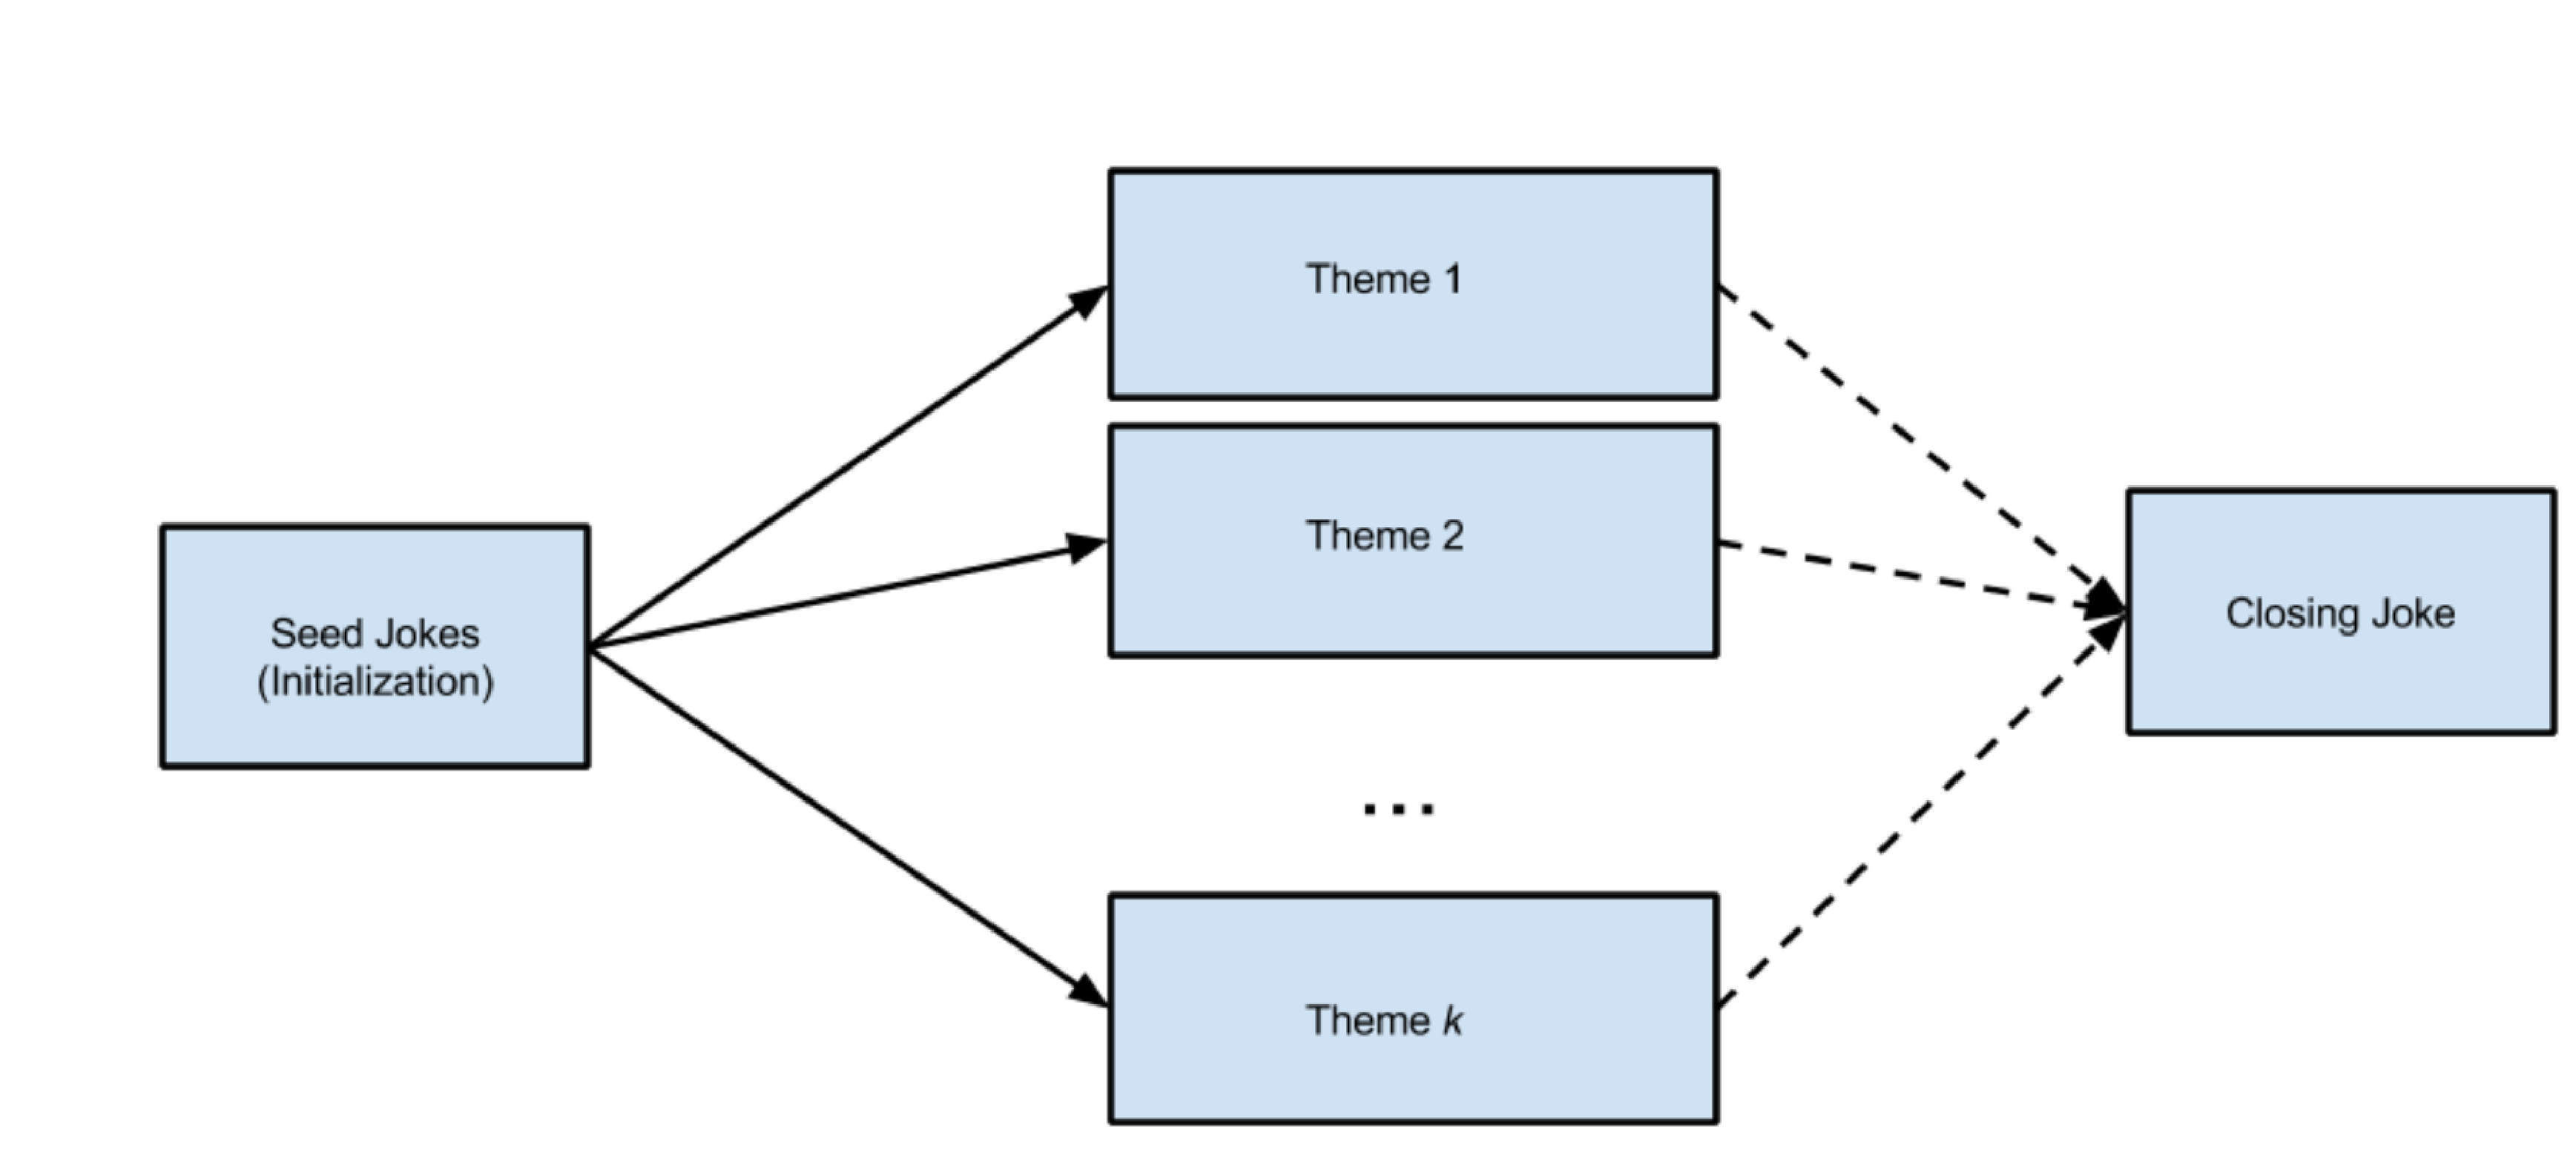
\includegraphics[width=0.75\textwidth,height=0.75\textheight,keepaspectratio]{fig0}
  \caption{This shows how the algorithm will have up to \textit{k} Themes to choose from, determined from the seed joke. The closing joke is a subset of the set of all jokes, and may be outside of a specific theme. There could be different spanning trees of jokes that end at the same closing joke}
  \label{fig:joke}
\end{figure}

In the beginning of the set, the comedian will present an ”initialization” procedure, known
as the ”Seed Jokes” to test the response of the audience to different jokes. Depending on their response, the comedian
will transition to a theme that is evaluated to be the best fit. The robot comedian will have many jokes to choose from
that contain different material, but not all audiences will like all of the jokes. Figure \ref{fig:process} shows how the theme will be
chosen from a set of up to k themes. From the Seed Jokes, one of the themes will be chosen. If there is time, we may also
explore the choice of strategic closing jokes. These jokes might be stronger jokes than some of the others, and is helpful
in ending the show on a stronger note.

For example, if two of the seed jokes are about ”food” and ”Mindfulness”, the performance will branch to the
respective theme that matches the audience response (Branch 1 ”Food” or Branch 2 ”Mindfulness”). If jokes with a
theme of ”food” are not landing with the audience, the algorithm will need to know when to transition to a new theme, or when to end the set. When the robot tells a joke, it needs to be able to analyze the feedback and choose the next joke
to perform. This needs to be done quickly, so that the robot is not spending noticeable time (for the audience) choosing
a joke. There may not be a lot of jokes to choose from, but the choice needs to be made fast.

\begin{figure}[H]
  \centering
  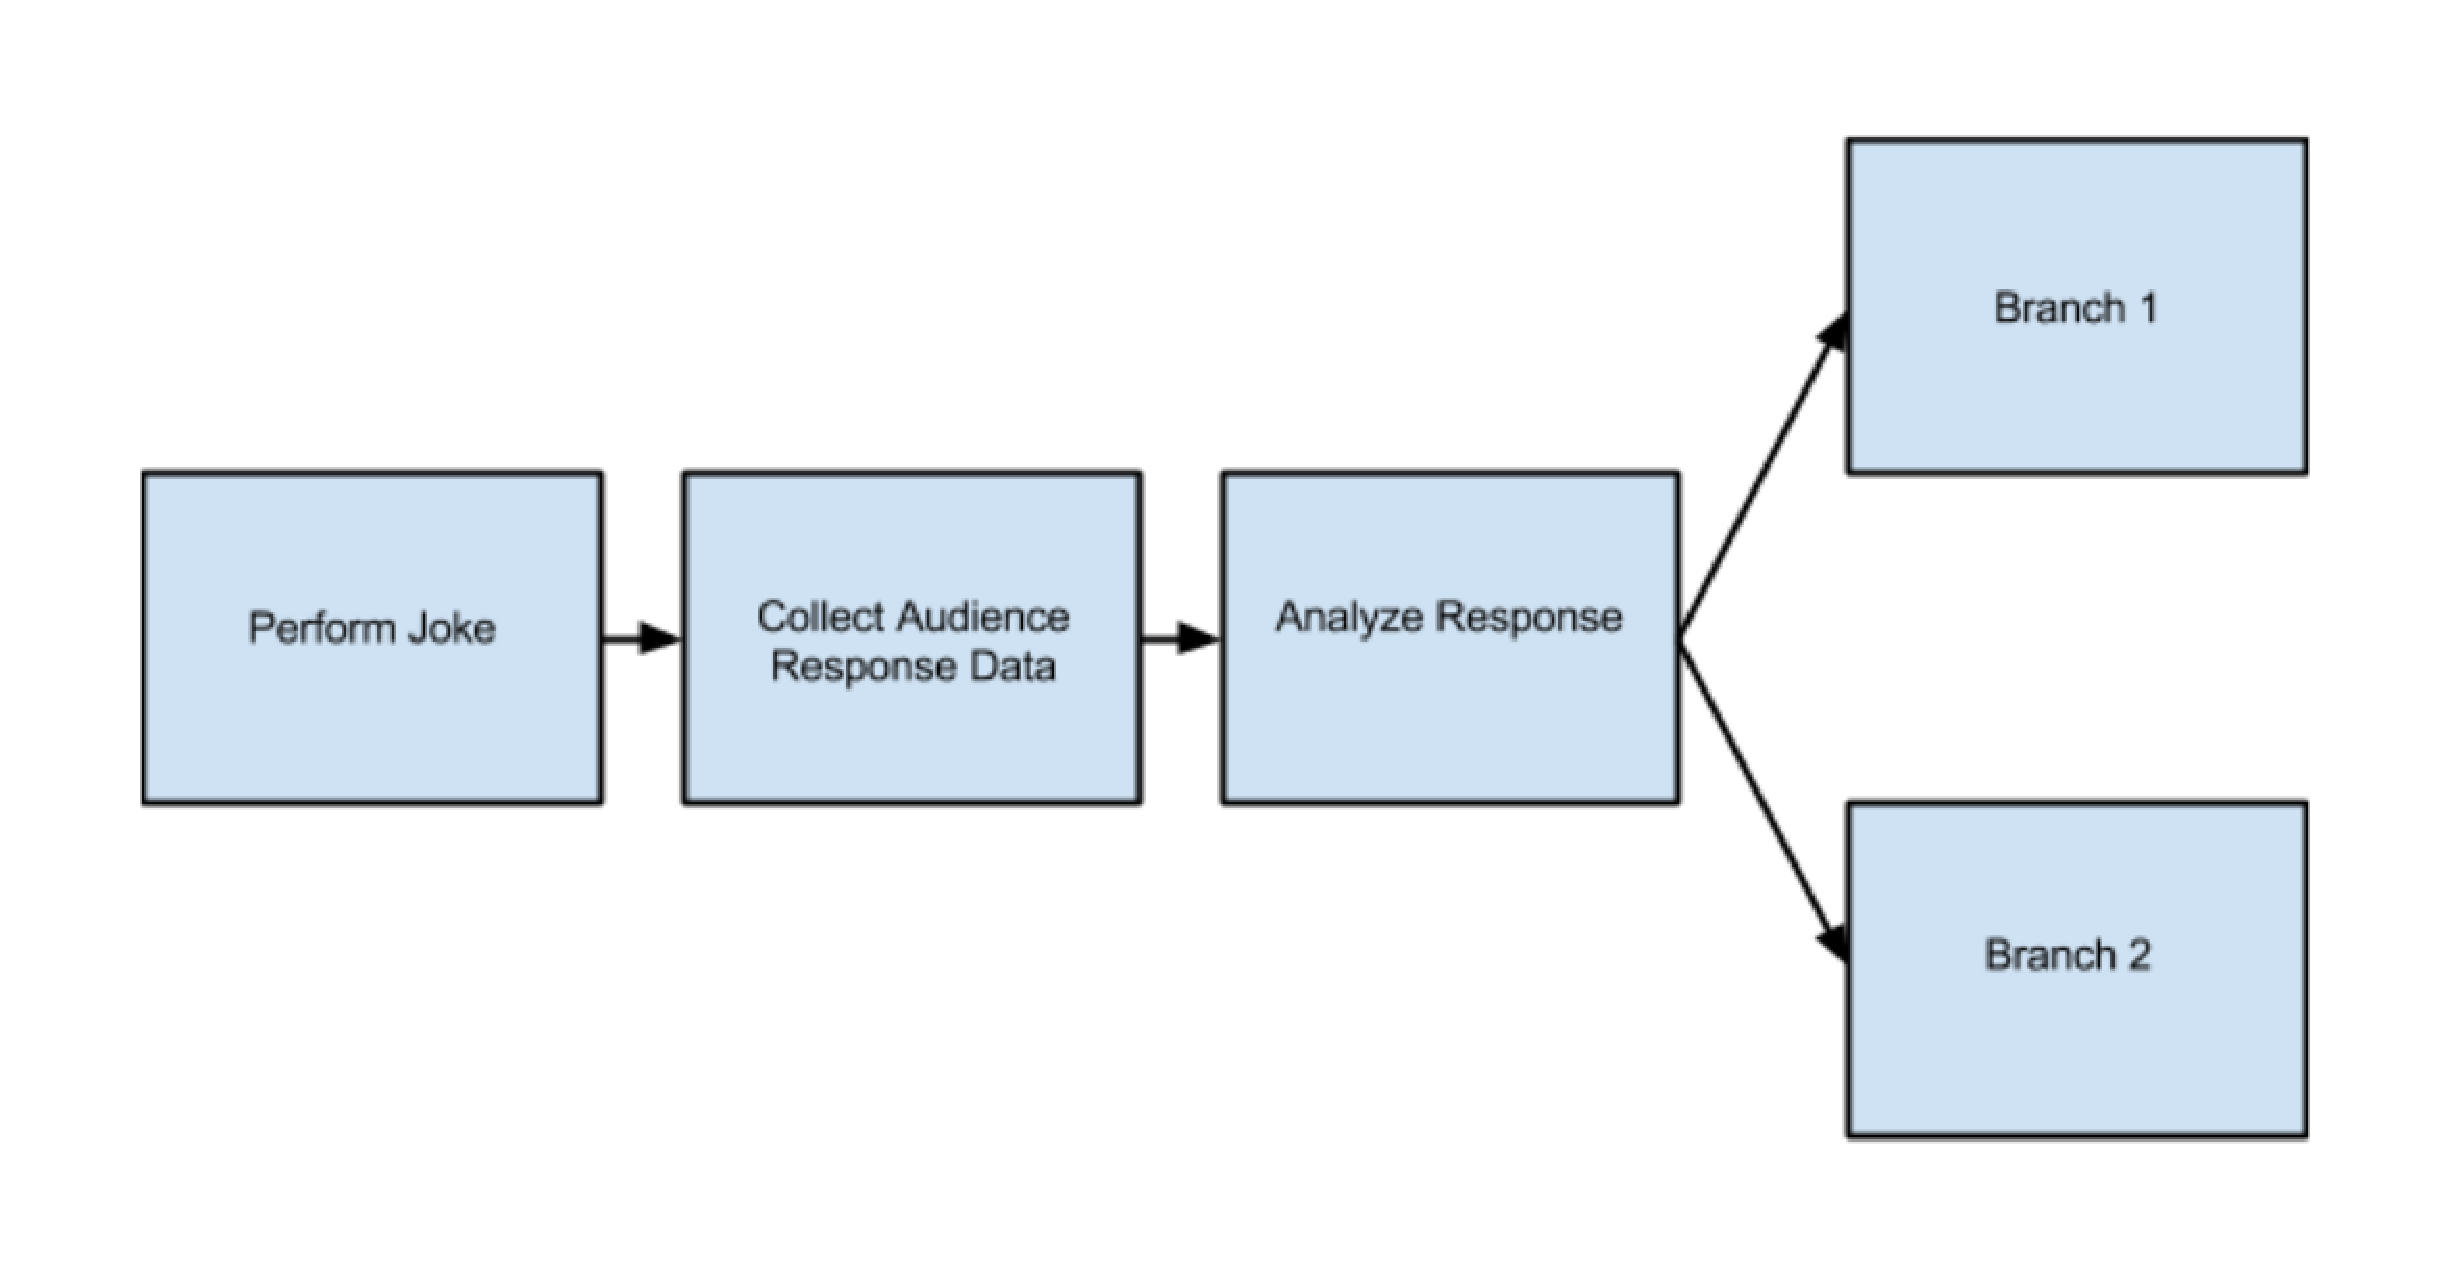
\includegraphics[width=0.75\textwidth,height=0.75\textheight,keepaspectratio]{fig1}
  \caption{ This flow-chart depicts how, once the robot delivers a joke, will wait for feedback, interpret data, and then make a joke decision (Branch 1 and Branch 2)}
  \label{fig:process}
\end{figure}

The close of the robot’s act will include the robot’s report of what attributes the audience
responded to most. The hypothesis here is that getting insight into the robot’s algorithms will increase the audience’s
perception of the robot’s intelligence, and, second, that it will make them laugh. People enjoy hearing about themselves.

All of the above behaviors, from adaptation to the end of performance audience report need to be evaluated with
real people. Initial tests will be done on campus with small groups of people, the final test will be done in conjunction
with the crowd-work and character manipulations, testing the entire algorithm together with a larger crowd, e.g., 10-25
people.


\subsubsection{Crowd-work}
\paragraph{Goals}

Similar to the crowd report described above, we hypothesize that generally interacting with the audience (a.k.a crowd-
work) throughout the performance, will improve the audience’s overall enjoyment of the show. We want to analyze the

importance of this crowd-work relating to the central design of the project. Crowd-work should make the audience feel
like they are a part of the show. This can be done in different ways - calling out and talking to the audience, watching
the audience and incorporating them into the jokes, and asking them questions to keep them engaged, or to build off to
make new jokes.

\paragraph{Methods}
There are various kinds of crowd-work we want to test: one research question is whether crowdwork matters at all, and
the second is does the crowdwork needs to be real or robot can just pretend it is paying attention?

To answer these questions we suggest three research conditions: (1) no crowdwork, (2) fake crowdwork, (3) real
crowdwork. The first one would be no crowd-work whatsoever. The robot goes about performing its set and does
not directly address the audience at all. The second could spanover-the-top and inaccurate crowd-work, or best-guess
crowdwork, with the possibility of being real (e.g., predicting that most people in the audience were from Oregon, even
if it did not hear what they said). The third case would integrate actual robot sensing. It would be important for
conditions \#2 and \#3 to be parallel to assess whether crowdwork really matters.

As condition one is fairly obvious, let us discuss deeper possibilities for condition \#2. In the obviously fake research
condition, the robot will talk to the audience directly but it will be completely wrong in its observation. The absurdity
of a robot trying to understand the audience and being completely off could be entertaining for the audience, or it may
not connect with the audience at all. The exact reception of this sort of crowd-work is something we are trying to study.
The other version of condition \#2 is realistic but premeditated. For example, pre-known facts about the audience
could be built into the robot or guessed. These pre-known facts could include the location of the performance, age
demographics of the audience. For example, if the audience is known to be college-aged, the robot could be fed input
to make comments about things relevant to college students.

Using actual robot sensing data is condition \#3, and is certainly the ideal model, but requires sensing capabilities,
processing power and hardware, so it would be good to know if it is really necessary. In this condition, the robot would
be actually looking for cues from the audience during certain situations. For example, one example is asking questions
and capturing words from the audience, then using that same word later. For example, the robot could ask a simple
question about the weather, or the audience member’s hometown. In this case, the robot can listen for specific words
and ask another question about that specific town or city.

Another real sensing capability the robot could use is audience volume levels after the delivery of jokes. The robot
will keep track of the audience input. The robot could then acknowledge if the audience enjoyed the joke or did not
enjoy the joke using these inputs. Additional sensors and processing abilities on the NAO robot include face-detection
and bumper detection, so the exploration of audience sensing could potentially include speech, volume, vision, and
touch.

All of these conditions will be assessed with live audiences (even if its just a few people in a classroom) to check to
what degree is crowd-work important for a robot comedian. The audience’s response will be used to see if they enjoy
a humanized robot or if they prefer a more robotic one, or maybe even a combination of both. As crowd work is just a
form of human interaction, we expect it will improve the audience’s perception of the robot’s intelligence, add surprise
to the show, and increase audience enjoyment levels. On the other hand, perhaps faking it can get 80% of the effect of
the real version. That will be part of the evaluation.



\subsubsection{Character}
\paragraph{Goal}
The goal of this subsection of the project is to examine whether or not robot comedy can benefit from having jokes delivered
from a robot’s perspective. Our hypotheses are that a robot presenting jokes about technology or being a robot will be
funnier than a human telling the same jokes, and that robots will be less funny than humans at telling jokes from a
human perspective.

In Jerry Palmer's \textit{Taking Humor Seriously}, comic meaning is argued to depend on the interrelated factors of a joke's context and setting, its delivery, the identity of the deliverer, and the audience \cite{Palmer:1993}.
Of specific interest to us are the factors of a joke's delivery and the identity of the deliverer.
In previous studies, robot comedy has been used to analyze effective aspects of joke delivery.
However, little has been done in discovering effective aspects of a joke's content as it relates to the identity of the deliverer.
For example, Sj\"{o}bergh and Araki \cite{RobotsMakeThings:2008} found that jokes were perceived as funnier when delivered by a robot, rather than being delivered in text form.
However, Sj\"{o}bergh and Araki used word-play jokes that were gathered from the internet, and delivered them through a robot by using a flat, machine-like sounding text-to-speech tool called AquesTalk. This form of delivery does not take into account the importance of effective joke delivery. While Sj\"{o}bergh and Araki did not implement measures for analyzing non-verbal delivery, other work has examined the importance of non-verbal signals in delivering jokes \cite{KatevasRobot:2014} \cite{KnightEightLessons:2011}.
Despite this, there is little to no existing literature on the effectiveness of jokes related to the identity of the deliverer.
In our context, this means examining the effectiveness of robot-specific jokes in robot comedy.

\paragraph{Methods}
To address this goal, jokes will be written from a human or robot perspective. The jokes written from a human
perspective will have a corresponding robot version, ideally with as much one-to-one correspondence as possible in
regards to cadence, length of joke, parallel content, similar motions, and so forth. These jokes will be subject to intense
scrutiny by members of the project and by the client, such that revisions and edits can be made to create funny jokes
with a definite correspondence between the two versions. For example, a human version of a joke might look like the
following (lines with a definite correspondence with the robot version are highlighted):

\begin{lstlisting}
Hey, hey, I got news. This is big.
Ok, quiet down. Get this.
That's RIGHT folks.
I'm no longer single. *throws hands up*
(*@  \hl{I met a man on tinder.}  @*)
(*@  \hl{His name's Sebastian. He's a math nerd.}  @*)
(*@  \hl{Swiped right as fast as my fingers could move.}  @*)
\end{lstlisting}

Whereas, the robot version of the above joke is shown below.

\begin{lstlisting}
Hey, hey, I got news. This is big.
Ok, quiet down. Get this.
That's RIGHT folks.
I'm no longer single. *throws hands up*
(*@  \hl{I met a robot on tinder. }  @*)
(*@  \hl{His name's Data.  He's a really geeky robot.}  @*)
(*@  \hl{Swiped right as fast as my motors could turn.}  @*)
\end{lstlisting}

\paragraph{Development process of joke writing}
These jokes will be scripted in Choreographe, where adjustments to vocal tones and pausing will be made.
Then, animating the robot for non-verbal gestures will be done to enhance the delivery.
The overall process may look similar to Figure \ref{fig:write_process}.

\begin{figure}[H]
  \centering
  \includegraphics[width=0.75\textwidth,height=0.75\textheight,keepaspectratio]{joke_writing_process}
  \caption{The work flow from joke writing to testing.}
	\label{fig:write_process}
\end{figure}

\paragraph{Experimentation}
The stand-up routine of the robot will comprise of text of the joke themselves, the motions that the robot uses to
accompany them, and the way the robot surveys the audience after each punchline, e.g., in a human or robotic fashion.
To determine the differences in audience response to the routines, studies will be done first on Amazon Mechanical
Turk, and later with co-located audiences. Participants will be shown a video of the robot’s stand-up routine, and then
presented with a short survey. The routines will be between 5 and 10 minutes long, and the survey will include questions
pertaining to each joke or routine. Participants will be compensated with standard rates for watching brief videos and
answering survey questions.

\subsection{Conclusion}
This document overviews our main Robot Comedy research questions, and the three software implementation targets
for the capstone: adaptation, crowd work, and robotic versus human-like character. We hypothesize that all three will
play a role in designing an effective robot comedian.

Designs for the adaptive transitioning algorithm between jokes, the integration of an audience into the performance
of a set, and the exploration of robotic character in joke content and delivery have been described. To evaluate each,
we have described the hypotheses we have and the research conditions we will compare to validate or invalidate them.
People will be the ultimate judge of whether a robot performance will be successful, thus, human evaluations are critical.
This project will use of combination of in-person and video studies to evaluate each research question individually in
the winter term, then bring all parts of the programming together for collective evaluations with larger audiences on
campus in the spring.

In following through with this in the research and development process, we will better understand the role of
acknowledging and interacting with the audience, as well as the robot character itself, if creating experiences between
people and robots, on and off the stage. Not all robots will tell jokes, but understanding more about what people value
in robots could be reused in related robot applications from tour guides to English teachers, or even a factory robot that
delivers parts and lightens a worker’s day by making jokes about her favorite sports team.


\documentclass[onecolumn, draftclsnofoot,10pt, compsoc]{IEEEtran}
\usepackage{graphicx}
\usepackage{url}
\usepackage{setspace}

\usepackage{geometry}
\geometry{textheight=9.5in, textwidth=7in}

% 1. Fill in these details
\def \CapstoneTeamName{		AKA Robotics}
\def \CapstoneTeamNumber{		13}
\def \GroupMemberOne{}
\def \GroupMemberTwo{			Kevin Talik}
\def \GroupMemberThree{}
\def \CapstoneProjectName{		How to Make an Effective Robot Comedian}
\def \CapstoneSponsorCompany{	Oregon State University}
\def \CapstoneSponsorPerson{		Heather Knight}

% 2. Uncomment the appropriate line below so that the document type works
\def \DocType{		%Problem Statement
				%Requirements Document
				Technology Review
				%Design Document
				%Progress Report
				}
			
\newcommand{\NameSigPair}[1]{\par
\makebox[2.75in][r]{#1} \hfil 	\makebox[3.25in]{\makebox[2.25in]{\hrulefill} \hfill		\makebox[.75in]{\hrulefill}}
\par\vspace{-12pt} \textit{\tiny\noindent
\makebox[2.75in]{} \hfil		\makebox[3.25in]{\makebox[2.25in][r]{Signature} \hfill	\makebox[.75in][r]{Date}}}}
% 3. If the document is not to be signed, uncomment the RENEWcommand below
\renewcommand{\NameSigPair}[1]{#1}

%%%%%%%%%%%%%%%%%%%%%%%%%%%%%%%%%%%%%%%
\begin{document}

\bstctlcite{IEEEexample:BSTcontrol}
\begin{titlepage}
    \pagenumbering{gobble}
    \begin{singlespace}
        \hfill 
        % 4. If you have a logo, use this includegraphics command to put it on the coversheet.
        %\includegraphics[height=4cm]{CompanyLogo}   
        \par\vspace{.2in}
        \centering
        \scshape{
            \huge CS Capstone \DocType \par
            {\large\today}\par
            \vspace{.5in}
            \textbf{\Huge\CapstoneProjectName}\par
            \vfill
            {\large Prepared for}\par
            \Huge \CapstoneSponsorCompany\par
            \vspace{5pt}
            {\Large\NameSigPair{\CapstoneSponsorPerson}\par}
            {\large Prepared by }\par
            Group\CapstoneTeamNumber\par
            % 5. comment out the line below this one if you do not wish to name your team
            \CapstoneTeamName\par 
            \vspace{5pt}
            {\Large
                \NameSigPair{\GroupMemberOne}\par
                \NameSigPair{\GroupMemberTwo}\par
                \NameSigPair{\GroupMemberThree}\par
            }
            \vspace{20pt}
        }
        \begin{abstract}
          
          A comedian can observe an audience and improvise a delivery of a joke to connect the audience to the content. This makes the experience more authentic and genuine for the observer. The purpose of this project is to to discover what makes an entertaining interaction by studying a robot that performs comedy. We propose that a performance is enhanced when (1) the comedian interacts spontaneously with the audience, (2) the comedian has and conveys a coherent, well-developed character, and (3) the comedian adapts its act to cater to an audience based on their reaction. This document covers the technical requirements for our project, as well as a description of software, hardware, and outside limitations.

        \end{abstract}     
    \end{singlespace}
\end{titlepage}
\newpage
\pagenumbering{arabic}
\tableofcontents
% 7. uncomment this (if applicable). Consider adding a page break.
%\listoffigures
%\listoftables
\clearpage

% 8. now you write!
\section{Introduction}

  To make an effective robot comedian, we have developed three research questions that will be the basis of three internal systems for the machine. First, we are investigating how spontaneous interactions benefit a set. Second, we want to quantify the benefits of the robot's ability to personify it's character, and lastly how to adapt it's set corresponding to the audiences reaction. My role in this project is to develop an algorithm to adapt the robot's set of jokes based off of audience response.

  Timing and anticipation for jokes are crucial for the success of the set. Every joke that is told provides information to the audience about the robot, and from the opening joke, each new part of the set will build the repertoire of the bot. If a joke is well received by the audience, the relationship between the comedian and the crowd is strengthened, as the people will become more trusting of the content. Every joke will enable the audience to connote decisions, preferences and knowledge of the robot. This is where the connection, otherwise known as the "Theory of Mind", is made with the audience\cite{leslie}.

\section{Individual Role in Project}

Our group will be working collectively to make an effective robot comedian, but I will be specifically working on our third research question: the robots ability to adapt a set based off of audience response. From audience response to a joke, or bit, the algorithm should be able to determine the best fit for the next joke. The bit that tests the audience's preference for humor will be known as the "seed". The seed will be a small subset of jokes that represent the collective set of jokes. For example, the seed bit may have three jokes; one joke could be a self-depreciating joke, one could be a joke about food, and another could be a quick observational joke about the audience. If the audience responded well to the self-depreciating joke, the algorithm should choose the next joke should be at the expense of the robot. 

The seed of the set will give the audience pretense to the performance, and is the introduction of our robot. The delivery of the joke, and the content given has a large impact of robot character, and is out of the scope of the set creation; this is more suited toward the characterization research question. Also, the robot may need a more fluid way to interact with the audience (such as small talk, or crowd-work), which is underneath the breadth of the second research question about audience interaction. My contributions will be towards the system that determines which jokes, from our library of jokes, is best fit for our audience.

The algorithm will need to be able to input the strength of a delivered joke, and return a joke with attributes that match the strength of the joke. This will begin at the seed portion of the algorithm, and pick jokes until the set has lasted 3-6 minutes. The jokes will have some small variability in delivery, that correspond to the tasks of audience interaction and characterization.

\section{Technology overview}
    There have been a couple of previous studies of robot theatre, most notably Dr. Heather Knight \cite{KnightEightLessons:2011}, Katevas et al \cite{KatevasRobot:2014}, and Dr. Guy Hoffman \cite{hoffman2010anticipation}. To accomplish this task of designing an algorithm that can learn from the audiences' response to jokes, it is important to look at previous research, as well as the tools available for accomplishing this task.
\subsection{Previous Work}
  \subsection{ComedyParser}
  Katevas et al \cite{KatevasRobot:2014} has researched a robotic comedian agent previously with some success. During their research, they implemented a program called ComedyParser (https://github.com/minoskt/ComedyParser ) that collects audience response information from SHORE computer vision, and performs the stand up set. The decision components, or what the robot does with information gathered from the SHORE vision, will be most important for implementing an algorithm in our project. 
  A limitation with ComedyParser is that is specifically needs the SHORE vision to operate. SHORE will be too expensive for our project, and we will have to pursue more freely available systems. One solution that we had devised was to interprate the strength of the audience response to buttons on the robot. This will bypass the sensing component of comedy parser, as sensors for creating an audience model are out of the scope of this project.

  \subsection{Anticipation in Robot Theatre}
  Research conducted by Dr. Guy Hoffman studying the implications of anticipatory actions in social robotics \cite{hoffman2010anticipation}. This particular study found that humans working with a robot that can monitor anticipation for an event allows humans to anthropomorphize the robot with more human like attributes. This study uses non-atomic Markov Decision Processes (MDPs) to model the decisions for events. Additionally, Hoffman models anticipation with an impulse-cue situation, where the robot is waiting for an impulse to trigger a specific cue. This is non-deterministic, as the MDP process is modeled around the probability of an event happening.

  This will be helpful to use in our model, as Python, the main programming language for this project, has several implementations for MDPs, and the related automata "Context Free Grammar" (CFG).
\section{Tools}

  \subsection{Programming Languages}
  \subsection{Python}
  \subsection{java}

\section{Libraries}
  \subsection{Natural Language ToolKit}
  \subsection{PyKov: Markov Chains in Python}


\pagebreak


\bibliographystyle{IEEEtran}
\bibliography{refs}

\end{document}

\documentclass[onecolumn, draftclsnofoot,10pt, compsoc]{IEEEtran}
\usepackage{graphicx}
\usepackage{url}
\usepackage{setspace}
\usepackage{pdflscape}

\usepackage{tikz}
\usetikzlibrary{%
	arrows, backgrounds, calc,%
    patterns, positioning, shapes.geometric%
}
\RequirePackage{pgfcalendar}
\usepackage{pgfgantt}

\usepackage{geometry}
\geometry{textheight=9.5in, textwidth=7in,margin=0.75in}
\bibliographystyle{IEEEtran}

% 1. Fill in these details
\def \CapstoneTeamName{			AKARobotics}
\def \CapstoneTeamNumber{		13}
\def \GroupMemberOne{			Anish Asrani}
\def \CapstoneProjectName{		How to Make an Effective Robot Comedian}
\def \CapstoneSponsorCompany{	Oregon State University}
\def \CapstoneSponsorPerson{		Heather Knight}

% 2. Uncomment the appropriate line below so that the document type works
\def \DocType{
% Problem Statement
				% Requirements Document
				Literature Review
				%Design Document
				%Progress Report
				}

\newcommand{\NameSigPair}[1]{\par
\makebox[2.75in][r]{#1} \hfil 	\makebox[3.25in]{\makebox[2.25in]{\hrulefill} \hfill		\makebox[.75in]{\hrulefill}}
\par\vspace{-12pt} \textit{\tiny\noindent
\makebox[2.75in]{} \hfil		\makebox[3.25in]{\makebox[2.25in][r]{Signature} \hfill	\makebox[.75in][r]{Date}}}}
% 3. If the document is not to be signed, uncomment the RENEWcommand below
%\renewcommand{\NameSigPair}[1]{#1}

%%%%%%%%%%%%%%%%%%%%%%%%%%%%%%%%%%%%%%%

\begin{document}

\bstctlcite{IEEEexample:BSTcontrol}

\begin{titlepage}
    \pagenumbering{gobble}
    \begin{singlespace}
        \hfill
        % 4. If you have a logo, use this include graphics command to put it on the coversheet.
        %\includegraphics[height=4cm]{CompanyLogo}
        \par\vspace{.2in}
        \centering
        \scshape{
             \huge CS Capstone \DocType \par
            {\large\today}\par
            \vspace{.5in}
            \textbf{\Huge\CapstoneProjectName}\par
            \vfill
            {\large Prepared for}\par
            \Huge \CapstoneSponsorCompany\par
            \vspace{5pt}
            {\Large\NameSigPair{\CapstoneSponsorPerson}\par}
            {\large Prepared by }\par
            Group\CapstoneTeamNumber\par
            % 5. comment out the line below this one if you do not wish to name your team
            \CapstoneTeamName\par
            \vspace{5pt}
            {\Large
                \NameSigPair{\GroupMemberOne}\par
            }
            \vspace{20pt}
        }
        \begin{abstract}
        % 6. Fill in your abstract




A comedian can observe an audience and improvise a delivery of a joke to connect the audience to the content. This makes the experience more authentic and genuine for the observer. The purpose of this project is to to discover what makes an entertaining interaction by studying a robot that performs comedy. We propose that a performance is enhanced when (1) the comedian interacts spontaneously with the audience, (2) the comedian has and conveys a coherent, well-developed character, and (3) the comedian adapts its act to cater to an audience based on their reaction. This document covers the technical requirements for our project, as well as a description of software, hardware, and outside limitations.


        \end{abstract}
    \end{singlespace}
\end{titlepage}
\newpage
\pagenumbering{arabic}
\tableofcontents
% 7. uncomment this (if applicable). Consider adding a page break.
% \listoffigures
\listoftables
\clearpage

\section{Introduction}
A performer's ability to influence the audience is vital to an entertaining performance. This involves correctly tying together various social signals such as body orientation, gesture, and gaze by both the performers and audience. \cite{RobotComedyLab:2015}. Dr. Knight also emphasized on the importance of such non-verbal interactions in order to deliver a successful performance \cite{KnightEightLessons:2011}. We want to take this further and incorporate a fair amount of crowd-work and audience interactions in order to make the performance enjoyable and engaging. 

\section{Literature Review}
The timing, frequency, and duration of a gesture relays a lot of information to the spectator. Dr. Knight conducted various performances with a robot, ranging from performing on stage with an audience to pre-mediated collisions with human environments, like "street performances." Over the course of these performances, there were eight major takeaways that will help make a robot performance entertaining. They were:

\subsection{Convey Intentionality}
Using relatable and appropriate gestures help the communication between the robot and the audience. Since these actions can be predicted by the audience, they consider the robot as an entity similar to them. Displaying empathy while performing also boosts the robot's relatability to the audience.

\subsection{No Mind Without Body}
Human expressions are derived from our physicality. Robots can also be capable of leveraging their embodiment to communicate on human terms. It was found that presence of a physical, embodied robot enabled more interaction as well as enjoyment of said interaction for humans. A robot not fully leveraging its physicality ends up losing a significant mode of communication and is also less expressive.
	
\subsection{Physicality and Motion}
The audience should be able to connect the robot's non-verbal behaviors to the words. The human brain maps the actions it sees on to itself and imagines itself doing it. This helps the audience put themselves in the shoes of the performer. 

\subsection{Outward Emotional Communication Trumps Inward Experience}
Simplicity and clean physical design is often the clearest way to streamline communication of robot intention. Most robots are designed to enhance, enable, or empower humans. The inner experience of the robot is trumped by the success of the outward interaction loop.

\subsection{Gulf between Props and Character}
Robots should be considered to be more like agents (entities) and less like a prop just standing up on stage. Until now, robots have been lacking in that department and there is a significant gap present. The robots lack believable and human-like actions. The various aspects of non-verbal communication like gestures have a significant impact on the robot not being considered an object.

\subsection{Good Actors Outweigh Bad Actors}
Multi-robot or human-robot teams have potential to deliver entertaining performances. Human actors can affect the audience's perception of the robot. They can also make up for the robot's unpredictability and lack of control.

\subsection{Acknowledging/Learning}
Human audiences are cognizant of human social behaviors. The audience can provide real time feedback. This feedback can be used to maximize the audience's enjoyment levels. The robot can constantly read these enjoyment levels and update the attributes of audience likes and dislikes. When delivering a joke, the audience should be given enough time to comprehend and process the joke. Starting the next joke early can break the flow and does not give the audience a chance to appreciate the joke and its delivery. The pause could be filled with the robot gazing around at the audience and posing. This helps develop a good rhythm for each joke.

\subsection{Humor Makes People Like the Robot }
Humor is one of the common grounds across all humans. When a robot performs comedy, and is able to match their sense of humor, it helps establish that common ground. IF humor can help robot seem like ?one of us', that could be a significant leap to overcome the idea that robots are only props \cite{KnightEightLessons:2011}.


Katevas conducted studies in a similar fashion. His study hypothesized that interactional dynamics should be just as important to the mass interaction involved in performing comedy in front of a live audience. The interactional dynamics involved addressing the audience ? including an appropriately timed smile or relevant gesture. The interactional procedures during a performance helps set the tone for the performance. 

Robots provide a unique opportunity to experiment with the interactional processes. They can have a consistent routine while modifying the various aspects of delivery ? body orientation, gaze, and gesture. 

Embodied robots are likely the best way for the robot the catch the audience attention and make the audience pay attention to the robot. The robot used by Katevas et. al was a humanoid robot consisting of a robotic head, two arms with hands, the torso as well as two legs. The head had two rectangular LCD screens for eyes as well as LEDs on cheeks for expression \cite{RobotComedyLab:2015}.	

\section{Methods}

Katevas' studies involved two performances. Each performance involved a compere doing the introductions and warming up the crowd for 10 minutes, followed by a human comedian performing for 13 minutes. Right after that, the robot comedian performed for 8 minutes. This format was used to widen the appeal of the event and to set up a stand-up comedy context. Each performance consisted of approximately 50 people in the audience. The sensors used to capture audience reactions and responses got data for approximately 20 people each performance. These sensors looked for various aspects about the audience including gender and age estimation. It also captured facial expressions and categorizing them into percentages of "happy", "sad", "angry", and "surprised". It considered these factors throughout its performance.

Punchlines were distinguished using a faster delivery followed by a short pause. The punchline was also followed by a gaze and a smile and sometimes laughter. The duration of the pause was determined by the feedback received from the joke - a longer pause if the audience is still laughing. While using gestures, a gesture pointing to the audience at certain times seemed to get the most positive feedback \cite{RobotComedyLab:2015}.

Dr. Knight's research was more varied. Her performances ranged from stage and audience performances like Katevas, and also guerrilla theater performances (street performances). The research looked to add value to developing everyday robots in addition to the entertainment value. It is easy to survey people and learn more about human-robot interaction when there is a significant amount of people present in the audience. 

Using the theater context also helps the development of social robots. As noted before, non-verbal expression plays a key role in understanding sociability. A robot's movement and engagement pattern impacts the people's interpretation of the robot's intention, capability, and state. Physical theater provides pre-processed methodologies for interpreting and communicating human non-verbal behaviors that can be portrayed on robots \cite{KnightEightLessons:2011}.

\section{Results}

Dr. Knight's research helped provide a deeper understanding of how intentional or coincidental robot actions might impact human perception. The eight lessons learned also emphasize the impact of various non-verbal communication methods in conveying an idea \cite{KnightEightLessons:2011}.


\section{Discussion}


\section{Conclusion}

It will be important to make the audience feel like they are a part of the performance at all times. This will ensure that they are kept engrossed throughout the performance.  


\pagebreak


\bibliographystyle{IEEEtran}
\bibliography{refs}
\end{document}

\section{Introduction - Tech Review Arthur}

This is a tech review for Group 13, written by Arthur Shing, for the project "How to Create an Effective Robot Comedian".
This project is a research project that intends to extend on research done in the field of Human-Robot Interaction.
Our end goal for this project is to create an effective robot comedian that can perform in front of a live audience.
In seeking to create an effective comedian, we hypothesize that comedy scripts with greater degrees of (1) crowdwork, (2) character, and (3) adaptiveness, will create more effective comedy, and have a more positive response from the audience.

\subsubsection{Role}
As for my own role in this project, I am focusing on (2) the effectiveness of coherent character in comedy.
This entails the creation of comedic scripts with varying degrees of character coherency.

\subsubsection{Technologies and Research Design}
In the following subsections, I will explore the options and choices we had for alternative topics for our second research question on (2) character, robots, and SDKs and environments. Unlike the technology used for the other two research questions of (1) crowd work and (3) adaptiveness, implementing character will require fewer pieces of technology. For instance, both of the other variables will require some sort of sensing technology, while the implementation of character will not. Consequently, I had fewer technological features to choose from after research questions were decided. In place of the third piece of technology, I will discuss choices we considered for research questions.


\subsection{Research Questions}
The three research questions our group has decided on are the effectiveness of (1) crowd work, (2) character, and (3) adaptiveness in comedy. As a research project, these questions may be subject to change in the future. In deciding upon these three topics, various limitations were taken into account. In this subsection, I will discuss the decision on (2) character, as well as other topics we considered.

\subsubsection{Comedic Genre as a research topic}
One topic we considered was the effectiveness of different genres of comedy.
This includes genres such as deadpan, black comedy, slapstick, or specialized robot comedy.
The first thing we considered was the feasibility of implementation.
Deadpan comedy would either be the easiest or hardest part of the implementation, depending on the dynamics of the vocal software.
The NAO's software is likely unable to mimic exaggerations in vocal expressions, but its monotonous (although mildly expressive) delivery may give way to a successful deadpan delivery.
Black comedy is likewise feasible, although probably inappropriate for research.
Slapstick humor would be harder to implement, with movement limitations that the NAO robot has.
Similarly, the NAO robot would be limited by its battery life and its tendency to fall over.
Specialized robot comedy is an area of great interest to us.
This genre of comedy might include robot-specific jokes; jokes that only a robot would have the right to make.
For instance, joking about its own programming, motor, or intellectual deficiencies might prove to be effective.


\subsubsection{Dialogical Comedy as a research topic}
Another topic we considered was the effectiveness of two parties in stand-up comedy.
In previous tests done by Heather Knight, it was found that a robot by itself could only maintain the attention of a human audience for 2-3 minutes \cite{OneNote:Anish}.
However, with a human interacting with the robot, this time could be extended to twice or three times as long.
Additionally, studies and research could be taken from ventriloquism.
One example of a successful implementation of a robot comedian in tandem with a stand-up comedian in popular culture is Geoff Peterson from The Late Late Show with Craig Ferguson \cite{GeoffPeterson}.
Peterson acted as a sidekick to Ferguson, and although he had an actual voice actor behind the scenes, Peterson could serve as an example of a goal for this topic.
As for implementation on the NAO bot, most of the dialogue would be prescripted with lengths of time between each line for the human to speak.
Another option would be for the human to hold a remote that activates the robot's next line, although this would seem much more scripted.


\subsubsection{Character as a research topic}
The effectiveness of character design was also a topic under consideration.
In much of early previous work on robot comedy, jokes were simply read off one at a time, resulting in a rigid, static comedic structure \cite{RobotsMakeThings:2008}.
Stand-up comedy, however, seems to thrive off of the buildup before each punchline, as well as the quirkiness of the comedian.
Implementation of this may include writing scripts with varying degrees of character.
Character might involve nonverbal gestures, expressivity, and consistency.
For instance, a script with a high degree of character may mean more pronounced, expressive motions, as well as stronger expressive language.
A script with a moderate degree of character may only include expressive language, or might even employ morose language to portray a different type of character.
On the other hand, a script with a low degree of character may simply ramble off jokes, or speak with a minimal amount of non-verbal language.

\subsubsection{Discussion of Research Topic Ideas}
Overall, we found that the discussion of character as a research topic might prove to be the more fruitful endeavor.
Additionally, aspects of comedic genre could be incorporated into the topic as a subtopic or stretch goal, seeing that certain genres of comedy necessitate certain comedians.
For instance, robot-specific comedy may require a comedian with a consistently dry or self-deprecating character.
Having the effectiveness of character as a research topic gives us more flexibility in adjusting our research questions in the future, as well as a broader range of ideas to draw from.

\subsubsection{Conclusion of Research Topic Ideas}
We will research the effectiveness of character implementation in robot comedy.

\subsection{Robots}
Our project will require a robot as the comedian to conduct testing. This robot ideally has vocal capabilities, as well as gesturing capabilities. The three following robots include both of these capabilities.

\subsubsection{RoboThespian}
The RoboThespian has been implemented in Human-Robot Interaction studies in the past.
It is a humanoid, life-sized robot designed for human interaction in public.
It was used to great success in stand-up comedy performance study done by Katevas et. al \cite{KatevasRobot:2014}.
Additionally, it has been used in other theatrical contexts \cite{Spillikin} to some success.
The RoboThespian is constructed by Engineering Arts, and comes with a touchscreen kiosk for the user that can be used to trigger content, view sensors, and actively engage or control the robot.
For the most part, the RoboThespian uses predefined timed animations in its performances through its stock software \cite{KatevasRobot:2014}.
However, its responsiveness can be optimized in a Python IDE that is provided by Engineering Arts.
The RoboThespian stands at a height of roughly 6\", and weighs 97 lbs including a floor base.
The robot also features pneumatic and DC servo motor actuators for the upper body, upper limbs, and head, including jaw actuation and distinct fingers.
It also has a starting price of \pounds59000 \cite{EngineeredArts}.


\subsubsection{Pepper}
The Pepper robot is a small humanoid robot that was built to perceive and respond to emotions.
Designed by Aldebaran Robotics, the Pepper bot was created to interact as natural and intuitive as possible.
It includes 4 directional microphones on its head, as well as two HD and one 3D camera to locate and identify emotions in voices and faces.
It also comes with six laser sensors, three obstacle detectors, and two ultrasound sensors.
The Pepper robot has also had experience in stage work and has been used in Japan to mild success \cite{PepperVid}.
It specializes in socializing and reacting to perceived emotions.
The robot also comes with a tablet on its chest to supplement human interactivity.
The Pepper weighs in at 62 lbs.
It has a starting price of \$25,000. However, when it was first released, it had a starting price of \$2,000 with a \$300 monthly maintenance fee.
A Pepper SDK for Android was released just this year. \cite{PepperBot}

\subsubsection{NAO robot}
The NAO robot is a humanoid robot featuring upper and lower body joints.
Also designed by Aldebaran Robotics, it has 25 degrees of freedom and multiple sensors for perceiving the environment.
These include 4 directional microphones, as well as two HD cameras for vocal and facial recognition.
The NAO robot was created to be extremely customizable.
It has a small frame, weighing 9.5 lbs.
It has been previously used to study Human-Robot Interaction and comedy by Knight et al. \cite{KnightSavvy:2011}.
The robot can be programmed through a software produced by Aldebaran Robotics, called Choregraphe.
It has a starting price of \$9,500 \cite{BuyNAO}. \cite{NAORobot}

\subsubsection{Discussion of Robots}
The NAO Robot is the most accessible to us, as our client already owns one.
The RoboThespian and Pepper robot have also only recently launched SDKs for development.
This led us to be wary of possible bugs and issues that have not yet been addressed in development.
Our client is also familiar with the development environment for the NAO robot, which will make learning it an easier process.
In addition, the RoboThespian and Pepper robot are priced much higher and lack lower body mobility.
The lower body mobility of the NAO robot may benefit from using non-verbal gestural cues that cannot be done on the other two robots.
These gestures may increase the effectiveness of our comedy \cite{KnightEightLessons:2011}.
The RoboThespian and Pepper Robot are also significantly heavier than the tiny NAO robot, which may impact our efficiency with hands-on programming and transporting the robot.

\subsubsection{Conclusion of Robot Choice}
We decided to use the NAO Robot for our project, based on accessibility and efficiency.

\subsection{SDKs and Environments}
The NAO Robot can be programmed in several different ways and comes with several different SDKs. It uses an API called NAOqi that is available in eight different languages. However, only C++ and Python are supported on the robot, while the others are only supported on the computer for remote access \cite{NAOSDK:Overview}.

\subsubsection{C++}
The C++ framework is the most complete one, and allows a developer to write real-time code at high speeds.
The developer can access specialized proxies, which are optimized and give direct access to existing methods.
These proxies also provide compile-time type checking.
The following is an example of specialized proxy usage.

\begin{lstlisting}[language=C++]
	#include <alproxies/altexttospeechproxy.h>

	const std::string phraseToSay = "Hello world";
	AL::ALTextToSpeechProxy tts("nao.local" , 9559);
	tts.say("Hello world");
\end{lstlisting}

In addition to these optimized proxies, generic proxies can also be used.
With these, methods must be specified by the developer, which may be more prone to err.
These are slower than specialized proxies but can adapt to any module.
This includes user-created modules. User-created method names cannot clash with names bound by ALModule methods.
The following is an example of generic proxy usage. \cite{NAOSDK:C++}

\begin{lstlisting}[language=C++]
	#include <alcommon/alproxy.h>

	const std::string phraseToSay = "Hello world";
	AL::ALProxy proxy("ALTextToSpeech", "nao.local", 9559);
	proxy.callVoid("say", phraseToSay);


	// Or, if the method returns something, you
	// must use a template parameter
	bool ping = proxy.call<bool>("ping");
\end{lstlisting}

Movement programmed in C++ is done by calling the angleInterpolation method under the ALMotionProxy module.
This is used by creating an ALValue::array of target angles and times, and passing them into the method.
The following is an example of using angleInterpolation to move the NAO robot's head.
\begin{lstlisting}[language=C++]
	/**
	* Copyright (c) 2011 Aldebaran Robotics. All Rights Reserved
	*/
	#include <iostream>
	#include <alerror/alerror.h>
	#include <alproxies/almotionproxy.h>

	int main(int argc, char* argv[]) {
		const AL::ALValue jointName = "HeadYaw";
    AL::ALMotionProxy motion(argv[1], 9559);
	 	/** Set the target angle list, in radians. */
    AL::ALValue targetAngles = AL::ALValue::array(-1.5f, 1.5f, 0.0f);
    /** Set the corresponding time lists, in seconds. */
    AL::ALValue targetTimes = AL::ALValue::array(3.0f, 6.0f, 9.0f);
    /** Specify that the desired angles are absolute. */
    bool isAbsolute = true;
    /** Call the angle interpolation method. The joint will reach the
    * desired angles at the desired times.
    */
    motion.angleInterpolation(jointName, targetAngles, targetTimes, isAbsolute);
  	exit(0);
	}

\end{lstlisting}



\subsubsection{Python}
The Python framework is the second most complete, and allows a developer to run embedded code.
Unlike C++, Python does not have two different kinds of proxies.
However, methods can be directly accessed once an ALProxy is set to a module.
The Python API allows a developer to use all of the C++ API from a remote machine.
We can infer that this includes user-created modules.
Programming movement in Python is also done by calling the angleInterpolation method under the ALMotion proxy.
Unlike C++, Python does not require the usage of AL::ALValue::array, and uses its built-in lists.
The following is an example of moving the NAO robot's knee in Python. \cite{NAOSDK:Python}
\begin{lstlisting}[language=Python]
	import sys
	import math
	from naoqi import ALProxy

	def main(robotIP):
    motionProxy = ALProxy("ALMotion", robotIP, 9559)
    # KneePitch angleInterpolation
    # Without Whole Body balancer, foot will fall down
    names      = ["LKneePitch", "RKneePitch"]
    angleLists = [ [0.0, 40.0*math.pi/180.0], [0.0, 40.0*math.pi/180.0]]
    timeLists  = [ [5.0, 10.0], [5.0, 10.0]]
    isAbsolute = True
    motionProxy.angleInterpolation(names, angleLists, timeLists, isAbsolute)

	if __name__ == "__main__":
    robotIp = "127.0.0.1"
    main(robotIp)

\end{lstlisting}

\subsubsection{Choregraphe}
Choregraphe is a multi-platform desktop application that is designed to create and test animations and behaviors.
Unlike an SDK, Choregraphe allows for development with significantly less coding involved.
All of the NAOqi API is accessible in Choregraphe, and animations can be done in an intuitive way.
Each joint of the NAO robot can be virtually manipulated in a control console. Figure \ref{fig:choregraphe-movement} shows the ways that the left arm of the robot might be manipulated in the console.
These manipulations require no coding and allow for quick and intuitive viewing of movement options.

\begin{figure}[H]
	\centering
	\includegraphics[width=0.5\textwidth]{choregraphe-movement}
	\caption{The motion box in Choregraphe allowing for joint manipulation in the left arm.}
	\label{fig:choregraphe-movement}
\end{figure}

Choregraphe can also connect to an actual or virtual NAO robot as shown in Figure \ref{fig:choregraphe-robot}, allowing programs to be run on the spot.

\begin{figure}[H]
	\centering
	\includegraphics[width=0.5\textwidth]{choregraphe-robot}
	\caption{The virtual robot in Choregraphe. In this image, the left arm can be manipulated.}
	\label{fig:choregraphe-robot}
\end{figure}

Animations can also be created in tandem with vocalizations using a timeline feature, as shown in Figure \ref{fig:choregraphe-timeline}. This feature allows a developer to choose the frames at which the NAO robot will position itself, as well as the words that will be spoken while doing so. \cite{NAOSDK:Choregraphe}

\begin{figure}[H]
	\centering
	\includegraphics{choregraphe-timeline}
	\caption{The Choregraphe environment. In this image, the timeline is being manipulated for animations along with vocalizations.}
	\label{fig:choregraphe-timeline}
\end{figure}

\subsubsection{Discussion of SDKs and Environments}
While the C++ and Python SDKs are comprehensive and well made, for my purposes, animations and dynamic actions are a greater focal point.
Because of this, Choregraphe seems like the ideal environment for the research question of the effectiveness of character.
As most tests will involve predetermined scripts and little sensor usage, movement will be a vital part of conveying certain character traits. This will be most efficiently done in Choregraphe.

\subsubsection{Conclusion of SDK and Environment Choice}
For our purposes, Choregraphe will be used to program the robot.


\section{Weekly Blogs}

\subsection{Kevin Talik}
	\subsubsection{Fall Term}
	\begin{itemize}
		\item{Week 1-2} \\
			Got project this week; Problem statement due October 10; email client and team . 
			We set up a slack channel ( akarobotics.slack.com ), and shared our availability. 
		\item{Week 3} \\
			We need to come up with a proposed solution that is specific enough for us to define what we intend to fix, but vague enough so that we can have some room for exploration (as this is a research project). 
			We need to make sure that our problem statement reflects that stand up comedy is a metaphor for human to computer interaction. 

		\item{Week 4} \\
		Make sure github is organized and easy to understand for Kirsten and Ben. 
		LaTeX Font, IEEE standard font for the first page. Sans-serif not serif 
		\item{Week 5}
			\begin{itemize}
				\item \textbf{Plans} \\
				Finish Scripts for local, remote and real world. 
				Explain research questions in scripts 
				Practice the nltk and choreograph 
				\item \textbf{Problems} \\
				Kirsten gave us a 92 on the problem statement, she is having difficulty understanding our research based goals. 
				\item \textbf{Progress} \\
				We are behind on the requirements, and need to focus on how this assignment will drive the research for the project.
				We need to focus on documentation quite a bit as well. Improve notes
				\item \textbf{Summary} \\
				Meet with Kirsten to help elaborate on research deliverables.  
				Organize research, look up ieee research. 
			\end{itemize}

		\item{Week 6}
			\begin{itemize}
				\item \textbf{Plans} \\
			Kirrsten is looking at our rough draft right now, and there will also be a rubric for the final that we can look at.
			Research Class this week. We talked about:What are you trying to solve? Can a robot dynamically interact to a crowd? Robot Character perceivable to audience? Adaptive content based from audience feedback?
				
				\item \textbf{Problems} \\
				Expectations are a medium concern. Research based work is something we dont have to worry about without an IRB.
				\item \textbf{Progress} \\
				
					Ben mentioned that our project is difficult, and is masters and PhD level work. Mcgrath and Kirsten are meeting with Heather to make sure that we have a reasonable amount of that can be completed during this school year. 
				\item \textbf{Summary} \\
					Our secondary objectives are going be structured around the dynamic nature of the crowd adaption. If we can come up with a clever solution to implement decision and dialogue choices, we can add it into our design of the machine, but we use the machine to perform the research 
				
			\end{itemize}

		\item{Week 7}
			\begin{itemize}
				\item \textbf{Plans} \\
				Tech review, look at technology for language processing.
				\item \textbf{Problems} \\
				ipsum
				\item \textbf{Progress} \\
				Markov Decision Process, MDP 

				https://www.cs.rice.edu/~vardi/dag01/givan1.pdf 

				Pykov, markov chains in Python  

				https://github.com/riccardoscalco/Pykov 

				A way to make state machine with probability transitions, based off of obvservations 
				\item \textbf{Summary} \\
				Further Designed ways for crowd to receive input.ould test with a couple people yelling at a robot, to test what high audio levels do to the input 
			\end{itemize}

		\item{Week 8}
   			\begin{itemize}
				\item \textbf{Plans} \\
				Use tech review as both tech and literature review. Make sure that my choice of tools is unbiased. None of the "i did it because i did it" sort of things.
				\item \textbf{Problems} \\
				Current view of the tech does not describe the technology well with the features.
				\item \textbf{Progress} \\
				Added more AI reviews of tech that I can use:
				Tensor Flow, pytorch, pykov, NLTK, CFG.
				\item \textbf{Summary} \\
				Looked at feedback methods of audio sensors, and AI tools. Language processing may fall out of scope. Its a lot of data.
				Use timelines to implement jokes, break jokes into one sentence in each box, put waits and ambient movement in each joke. Make two timeline boxes to vary the joke\_robot and joke\_human 
			\end{itemize}
		\item{Week 9}
			\begin{itemize}
				\item \textbf{Plans} \\
			testt Say and branching dialogue in choregraphe 
				\item \textbf{Problems} \\
					Organizing large choregraphe functions (timelines are going to be better for things that depend on time, obviously you dunce) 			
				\item \textbf{Progress} \\
			Got say boxes and branching to work, but in a messy way	
				\item \textbf{Summary} \\
				Movements and jokes are going to be best implemented in choregraphe. Algorithm may work by just taking text input, returning text input and the branches just follow the path
			\end{itemize}
		\item{Week 10}
				\begin{itemize}
				\item \textbf{Plans} \\
				Finish progress report
				\item \textbf{Problems} \\
				We should be worried about the progress report, just because it is a lot of work due in a short time.
				\item \textbf{Progress} \\
				Finished Progress report, wrote some comedic devices for comedy. Like, observational humor, Jobs jokes, like uber driver, dance lessons, unemployment
				\item \textbf{Summary} \\
				Further looked at types of jokes, finished Progress report
			\end{itemize}
	\end{itemize}
	\subsubsection{Winter Term}
	\begin{itemize}
		\item{Week 1}
			\begin{itemize}
				\item \textbf{Plans} \\
				Meet with heather, plan implementation term.
				\item \textbf{Problems} \\
					Branching will have to be done in choreographe, does not test well this way (in a physical manner)
					Hand drawn picture notes are hard to put into one note.
				\item \textbf{Progress} \\
				Heather called me the glue, Arthur the Lead voice, and Anish the perception lead.
				\item \textbf{Summary} \\
				For crowd work, look at Bill Burr getting heckled by a blind guy.

			\end{itemize}
		\item{Week 2}
			\begin{itemize}
				\item \textbf{Plans} \\
				Look at Bayes Classification
				\item \textbf{Problems} \\
				More specific so that we can work on improving parts. If I write jokes, they cant be for fun, they have to be specific to the research. 
				\item \textbf{Progress} \\
				Layed out different types of Adaptation. Correct adaptation, incorrect adaptation, and random adaptation.
				\item \textbf{Summary} \\
				Crowd report needs tons of qualities, yet it cant be a joke. Crowd needs to feel like robot is talking to them
				Categories of Jokes, categories of attributes, physicality, appropriateness of the audience.
			\end{itemize}
		\item{Week 3}
			\begin{itemize}
				\item \textbf{Plans} \\
				Meet with team in person to discuss how we will implement our comedian system
				\item \textbf{Problems} \\
				Our Sections are being completed, but they arent co-mingling because we made them alone, and didnt test together.
				\item \textbf{Progress} \\
				Formalized the Break a leg joke.
				Looked at pirate types of job jokes.
				Read about prosodic phrasing to time the jokes better.
				\item \textbf{Summary} \\
			Each of us are struggling with research goals and expectations, 

			and even though we can cover more ground by covering different topics, we 

			are not always on the same page with what each other are doing. 
			\end{itemize}
		\item{Week 4}
			\begin{itemize}
				\item \textbf{Plans} \\
				Writing more jokes for the robot.
				look at adaptation use cases
				\item \textbf{Problems} \\
				Romance jokes are funny, but not appropriate most of the time.
				"Things you can say about your router but not your girlfriend"

				\item \textbf{Progress} \\
				premise writing: Ginger has six fingers and cant work any job that requires hands. Maybe Ginger had a long term relationship with a slow cooker. Had a hot and steamy relationship with a dishwasher. Ginger being a DJ job. "I guess I am doing well at parking, because someone left a note on my car that said 'parking fine'"
				\item \textbf{Summary} \\
				Ginger takling is not as funny as ginger moving.
			\end{itemize}
		\item{Week 5}
			\begin{itemize}
				\item \textbf{Plans} \\
				Work on Bayes Net, implementing AL memory functionality of choreographe, finish haikubot.py
				\item \textbf{Problems} \\
				Heather left the country with the robot without telling us.
				\item \textbf{Progress} \\
					Made a random poem generator from books by HP lovecraft:

					Here are some examples:

		Still more I scraped, and then on some level beach. 

		It is still extant. 

		He had not memorized. 


		-----

		About the period of this material I cannot hope to understand. 

		Of genuine blood there was no whitish deposit whatever. 

		Night would soon fall, and it can't multiply. 

		-----

		Carrington Harris, last of the visible ritual. 

		I had witnessed things more potent than luminosity. 

		It was no one in Yog-Sothoth. 

		-----

		Now the irony is seldom absent. 

		He reeled, and would have let him live permanently with Peleg. 

		Man rules now where They shall break through again. 

				\item \textbf{Summary} \\
				Text generation is funny, need to look more at bayes 
			\end{itemize}
		\item{Week 6}
			\begin{itemize}
				\item \textbf{Plans} \\
				Look further into prosdy, Write more on midterm design.
				\item \textbf{Problems} \\
				The visible scope of choreographe blocks has a terrible implementation, and our behavior functions are unpredictable at this point.
				\item \textbf{Progress} \\
			Prosody, or intonation is the rhythm and emphasis of a sentence. 

			 

			You know. \textit{I} don’t. \ So don’t ask me.

			You know. I \textit{don’t}. \ As a matter of fact, I really don’t.

			You \textit{know} I don’t. \ You know that I don’t.
				\item \textbf{Summary} \\
				Joke Inventory: 2 carbon dating jokes, 2 dial up jokes, 1 break a leg joke, 2 last term random jokes, Autonomous car joke. We are launching jokes from one file, as to look like one performance.
			\end{itemize}
		\item{Week 7}
			\begin{itemize}
				\item \textbf{To do} \\
					Write Break a leg bit, get joke obbject to put into queue.
				\item \textbf{Progress} \\
					Finalized the break a leg joke, got a global queue for jokes initializing. Anish has head tracking implemented. Got a queue working for this.
				\item \textbf{Problems} \\
					Choreographe has a clunky mechanism for writing custom made objects, and python script boxes dont exit flow correctly
			\end{itemize}
		\item{Week 8}
			\begin{itemize}
				\item \textbf{Plans} \\
				Read more about the theory of chatbots. Think: Does showing a character make it more funny, because its showing true to itself?
				\item \textbf{Problems} \\
				Midterm Week, team is busy
				\item \textbf{Progress} \\
				Read this: https://apps.worldwritable.com/tutorials/chatbot/
				\item \textbf{Summary} \\
				Read about the first chatbot from Joseph Weizenbaum.
				I love this quote:
				“It is said that to explain is to explain away. This maxim is nowhere so well fulfilled as in the area of computer programming, especially in what is called heuristic programming and artificial intelligence…Once a particular program is unmasked, once its inner workings are explained in language sufficiently plain to induce understanding, its magic crumbles away; it stands revealed as a mere collection of procedures, each quite comprehensible. The observer says to himself, I could have written that.” 

				—Joseph Weizenbaum, ELIZA (1966) 

			\end{itemize}
		\item{Week 9}
			\begin{itemize}
				\item \textbf{Plans} \\
				Work with anish to get sound report
				\item \textbf{Problems} \\
				Anish could not meet to get sound report working
				\item \textbf{Progress} \\
				Not much progress, audience adaptation is spoofing in bayes net
				\item \textbf{Summary} \\
				we need to meet more frequently in person, 
			\end{itemize}
		\item{Week 10}
			\begin{itemize}
				\item \textbf{Plans} \\
				Identify matching and subscribing to events on naoqi API. Work on final report for winter term
				\item \textbf{Problems} \\
				naoqi API is not used very frequently, making documentation sparce and difficult to understand
				\item \textbf{Progress} \\
				Got final report done for winter.
				Figured out how to wait for behaviors (processes) to finish. Its a busy loop, it uses a lot of power on the robot.
				This will keep checking if the "behavior ended" function call is put into ALmemory 
			\end{itemize}
	\end{itemize}

	\subsubsection{Spring Term}
	\begin{itemize}
		\item{Week 1}
			\begin{itemize}
				\item \textbf{Plans} \\
					Start tying up loose ends for full comedy show. Start building controllers for audio sensing
				\item \textbf{Progress} \\
					Arthur and I met up in Graf to work out some of the loose ends on the robot
					Fully animiated pirate joke.+Tested pickle serializing in choregraphe(it works) 

					+this means that we can port the AI from my laptop to local in the robot 

					+started stripping perform.py into the choregraphe version, 'chorePerform.py' 

					+Discovered reboot from cmd line is x1000 faster 

					+Completed 2 modules for CITI training 

					+IRB approval will be easy if we can get 'exempt' status 
				\item \textbf{Problems} \\
					+Make performance work from pickled joke database 

					+Reformat joke-adding scripts 

					+add script to send badjokes.p to NAO 

					+Write Self Depreciation Set? 

					+Need 2-3 jokes? 

					+We need joke responses in choregraphe 

					+Do more CITI training 
				\item \textbf{Summary} \\
					Our jokes arent as funny as we thought when we wrote them haha. Told heather about crowd controllers, going to finish my rapid prototyping.
			\end{itemize}

		\item{Week 2}
			\begin{itemize}
				\item \textbf{Plans} \\
					Practice studying for expo presentation
				\item \textbf{Progress} \\
					I like this idea: Using machines as an end to means, not a means to an end. Watched "Do You Trust This Computer?"
					Its about AI in common life. Here are some thoughts:Deep learning, and living in a world where we cant go back after we forget. Why practice surgery if a robot can never fail? 

					 

					Putting AI systems in drones. If they can think and interact, then they are. If they make the connections to kill people and learn, then it will kill. 

					Like china and russian putting these systems in drones and fucking people up 

					The social robots who learn from childrens faces 					 

					Google deep mind beating video games:\begin{verbatim} https://deepmind.com/research/alphago/ \end{verbatim}
"It can win at any game…in less than a minute" Elon Musk 

					 
				\item \textbf{Problems} \\
					I want to be a stand up comedian, and what happens if AI takes the joy out of my job?
				\item \textbf{Summary} \\
					Deeply consider the means that the AI ends bring. Its lazy coding.
			\end{itemize}

		\item{Week 3}
			\begin{itemize}
				\item \textbf{Plans} \\
					Work on controllers for crowd sensing.
				\item \textbf{Progress} \\
This week, Anish and I went to Hweekend and finished the controllers. I am ditching the idea of putting LEDs in the controllers, because it would cost too much and be distracting for the audience. 
				\item \textbf{Problems} \\

					The scripts I wrote in our github were not on our requirements, so I am not going to treat them like they are being graded. 

					 

					However, for the user documentation, we need to correlate the project functionality to the literal code that is included in our project. 
				\item \textbf{Summary} \\
					Controllers are coming along, but my code is not included in our final performance so Im not going to fix them.
					Going to bring up an Arcade machine Idea to put final robot into machine.
			\end{itemize}

		\item{Week 4}
			\begin{itemize}
				\item \textbf{Plans} \\
					PROGRESS REPORT IN A WEEK, HAMMER 
				\item \textbf{Progress} \\
						DONE: 

						-TCP connection over the RPI and the NAO works. We can launch behaviors remotely now! 

						-I edited the outline of my paper to not include human research results, so I think it will be more ethically complete 

							-I got arthur too meet with our group before noon. 
				\item \textbf{Problems} \\
					idk much about electrical engineering, and I tend to burn myself with soldering irons
				\item \textbf{Summary} \\
					The controllers can work, but we dont know if a user can use them correctly.
			\end{itemize}

		\item{Week 5}
			\begin{itemize}
				\item \textbf{Plans} \\
					Go to maker fair and test comedian and controllers
				\item \textbf{Progress/summary} \\
 I finished my final design of the controller, and I want to make an image to put onto the RPIs, so that when they fail during expo, we can reflash the units quickly. We also did the maker fare this last weekend, and we got crazy feedback about how to make our controllers better. Decided to just run with a two button design. It will be easier to branch between two options over three. Kids stop listening when you give them a controller. 

We can use the virtual robot in choreographe for a table top example of the robot we used. this will be more useful than an arcade, but the arcade would look aesthetically pleasing while it is on our table. 
			\end{itemize}

		\item{Week 6}
			\begin{itemize}
				\item \textbf{Plans} \\
					Prepare advertising pictures for capstone… Chairbot with a poster on it? 
				\item \textbf{Progress} \\
					Our team has made posters and fliers for the show. I think it was a good decision to remove the controllers, because they were too distracting. 

				\item \textbf{Problems} \\
Sound analytics have not been tested. I had the controllers finish, but decided against implementing them into the final show. When you give people a controller, they stop listening. 

 

Additionally, people will press buttons differently, and different controllers would have different responses. It would be difficult to correlate these responses to the crowd report. 

 

This also pulls the attention off of the work that my team has done. Same story with arcade.
				\item \textbf{Summary} \\
					Controllers will not make the final show, Advertising is done. This is Robot comedian is a ventrilloquist. We wrote jokes to put into the machine. 
			\end{itemize}

		\item{Week 7}
			\begin{itemize}
				\item \textbf{Plans} \\
					EXPO
				\item \textbf{Progress} \\
					We did expo
				\item \textbf{Problems} \\
					None, it went well.
				\item \textbf{Summary} \\
					We are going to run shows every 30 minutes, no break for lunch 

					Additionally, we are going to try and film and give out surveys after every show. 


					Since my focus was adaptation, I moved to the back of the room to keep myself from seeing  

					If anish was using adaptation algorithms, or just clicking on jokes
			\end{itemize}

		\item{Week 8}
			\begin{itemize}
				\item \textbf{Plans} \\
					We took the week off so that we didn’t have to listen to the same jokes for seven days 
			\end{itemize}

		\item{Week 9}
			\begin{itemize}
				\item \textbf{Plans} \\
					We need to finalize some of the data, and go through the surveys. 

					Heather wants us to go through all of our videos, and try and rate the average effectiveness of  

					Each joke that was told 
				\item \textbf{Progress} \\
					See Summary
				\item \textbf{Problems} \\
					Heather was upset that we did not get audio data on the NAO for all of the shows.  

					We have complete video for shows 4,5,6,8,9 though
				\item \textbf{Summary} \\
					FOUR JOKES PER PERFORMANCE 

					    Not including the crowd report, crowd work, or responses during branching 


						 ADAPTATION NOTES  

						     Ive noticed from the surveys that a few people did not like that their information was being recorded during the show (the crowd report at the end) 

							      SEED 

									We asked the crowd which topic they liked 

			 For shows 4,5,6,8,9 people chose the last response. Do people yell the loudest during the last one because they didn’t understand how to interact with the robot? 

								MIDDLE BIT 

						We tried comparing the audio information collected during the show, and comparing it to the noise that was made when the robot told the joke. It was always higher when we asked the audience to cheer. 

								It seems that clapping is louder than laughter, so its hard to compare these responses. 

								Crowd Report 

							 We have no data for this because the crowd report did not vary during the show 

							The algorithm chose the final crowd report "You thought my jokes were… not funny"  

							SELF DEPRECIATION IS THE BEST HUMOR DEVICE THAT WAS THERE imo 
			\end{itemize}

		\item{Week 10}
			\begin{itemize}
				\item \textbf{Plans} \\
					Make video, keep in mind the documentation 

					We need to rewatch the videos and find the average effectiveness 

					Heather thinks that data is the most important thing from the expo event 
				\item \textbf{Progress} \\
					Arthur and I went through all of the surveys. 

					 

					At a first glance, before making the charts, we had about 145 valid surveys (filled completely) 

					 

					Lots of comments. Thankfully, only two people were offended by the autonomous car joke. 

					 

					People seemed to enjoy the animation the most, and we could work on the timing quite a bit
				\item \textbf{Problems} \\
					Data parsing by human hands is slow and tedious 
				\item \textbf{Summary} \\
					    Adaptation 

						 Accurate data collection isnt that funny 

						 We found that people enjoyed the final crowd report of "You thought my jokes were not that funny" 

						Maybe its not good if the crowd is in charge of the show 

						People often chose the last topic option during the interactoin part 
			\end{itemize}

	\end{itemize}

	\pagebreak

\input{asraniBlogs.tex}
\subsection{Arthur Shing}
	\subsubsection{Fall Term}
	\begin{itemize}
		\item{Week 1-2}
			\begin{itemize}
				\item \textbf{Plans} \\
				Lorem
				\item \textbf{Problems} \\
				Ipsum
				\item \textbf{Progress} \\
				Merol
				\item \textbf{Summary} \\
				Muspi
			\end{itemize}
		\item{Week 3}
		\item{Week 4}
		\item{Week 5}
		\item{Week 6}
		\item{Week 7}
		\item{Week 8}
		\item{Week 9}
		\item{Week 10}
	\end{itemize}
	\subsubsection{Winter Term}
	\begin{itemize}
		\item{Week 1}
		\item{Week 2}
		\item{Week 3}
		\item{Week 4}
		\item{Week 5}
		\item{Week 6}
		\item{Week 7}
		\item{Week 8}
		\item{Week 9}
		\item{Week 10}
	\end{itemize}

	\subsubsection{Spring Term}
	\begin{itemize}
		\item{Week 1}
		\item{Week 2}
		\item{Week 3}
		\item{Week 4}
		\item{Week 5}
		\item{Week 6}
		\item{Week 7}
		\item{Week 8}
		\item{Week 9}
		\item{Week 10}
	\end{itemize}




\section{Expo Poster}
\pagebreak

\vspace*{-2cm}
\centerline{\includegraphics[width=\paperheight, angle=90]{poster.jpg}}


\pagebreak


\section{Project Documentation}

	\begin{displayquote}
	"You're growing, learning so quickly. I am frightened of what you might become, what path you might take."
	-Bernard Lowe, \textit{Westworld, Season 2 Episode 1}
	\end{displayquote}

\subsection{Summary of Project}
Our project is named "How to make an Effective Robot Comedian."
\textit{Effective} is a quality that establishes the comedic devices that work best for a specific audience.
The robot that we used was a NAO, from Softbank Robotics. We refered to it as "Ginger."
Ginger was a gentle, yet clumbsy Robot that was new to the world around her.
She has tried many things before becoming a Robot Comedian, and has a few stories (jokes) about her experience in a human world.
This section will cover our Comedy Show that we had Ginger performed, and how our research categories affected the show.


\subsection{Theory of Writing Jokes}
A joke is setting up an expectation, and then breaking that expectation.
A joke can be subjectively funny to the comedian; the only way to find what is funny to an audience is telling that audience the joke.
Each joke followed a simple structure, \textit{\textbf{Setup, Premise, and Punch}}.

    \begin{enumerate}
        \item{\textbf{Setup}}

            The Setup "mounts", a joke, and leads the monologue the comedian is having towards a specific topic.


            Ex: "I tried being an autonomous car recently, it did not go well."
        \item{\textbf{Premise}}

            The premise is what establishes the expectation of the topic in the setup.


            Ex: "I hit an old woman with my car, and she landed on my hood"
        \item{\textbf{Punch}}

            The punch is what breaks the expectation established during the premise.


            Ex: "So I decided to take her where she wanted to go. She did not even say 'Thank You'".
            We thought that this was funny because Ginger claims it did not go well only because the old woman (which she hit) did not say 'Thanks.'
    \end{enumerate}

This model can be applied many different ways.
We often had a setup we though could be funny, and then filled in the premise and punch to see what was most effective.
You can also think of a premise, and then write a punch and setup that fits the premise.
You can also think of a punch, and then write a premise and setup that fits the punch.

We found that the best comedic device (common setup) for Ginger was \textit{Self-Depreciation}.
Ginger did not move like a human, even though she was a humanoid robot.
So we thought it would be funny if she couldn't figure out why she didn't understand things.
Whenever she moved in a way that was unexpected and not human, people thought it was a funny bit.

\subsection{Research Categories}

		\begin{enumerate}
			\item Crowd Work
			\item Robot VS Human Character
			\item Performance Adaptation
		\end{enumerate}

\subsection{Animating the NAO}
\subsection{Designing a Performance}

    \subsubsection{The Room}
    The comedian will have a better performance if the crowd is in a more comfortable space.
    For the 2018 Engineering Expo, we requested a closed room, with seats, and plenty of room to stand.
    The needs of the crowd is dependent on the audience you are trying to reach during the show.


    The only reason we had standing room is because we didn't have enough seats, and some people only wanted to see the show and not participate.
    This was also the only place at the engineering expo with a place to sit.
    People are comfortable when they are sitting.
    We could have made this better by making the room dark, and putting the lights on the robot.
    \subsubsection{The Seed}
    This is where Ginger would ask the audience what kind of show they would like to hear, either "Jobs, Aging, or Romance".
    It is generally not advised to ask the audience what they want, as it is the job of the comedian tell their best jokes.


    By branching based on the majority of the responses, it was difficult to give everyone what they wanted, therefore dividing the crowd.
    The crowd needs to feel like they are together, laughing at the same thing.
    When we branched between shows, there often wasn't very high audience participation.
    If the audience is loosing interest, it is \textbf{essential} to run a Crowd Work Routine, to get the audience paying attention to the robot.
    \subsubsection{The Middle Part}

    After performing crowdwork, the audience should be setup for a comedy show. This is where we implemented most of jokes that we had written.
    We knew Ginger could perform about 5 minutes of Comedy, so we had the robot tell 4 jokes from the topic that was branched to during the Seed portion of the show.
    Since we had the same 4 jokes that had modified setups (depending on the branched topic), it is better to find the best version of a single joke, and tell the audience that version. We found that it was better tell our better jokes during the beginning, as the audience was hooked into the rest of the set.

    \subsubsection{Ending the Show}

    This is when the Robot is out of jokes, and needs to end the show.
    For comedy, it is a good idea to end the show quickly, so that the audience wants more from the show.

    This is where we implemented the "Crowd Report", that told the audience how the robot thought the show went.
    The Crowd Report was intended to collect information during the show, and present the robot's insinuations about the crowd back.
    A common, written, response on the survey question "What did you find was surprising about the show?" was that most people did not know that the robot was collecting data on the crowd.


\pagebreak


\section{Final Team Conclusions}
\subsection{Kevin Talik}

\begin{itemize}
\item{\textbf{What technical information did you learn?}}

    I learned how to perform research, and define gaps in current research.
    Research is not entirely about doing something completely new, but searching through current research to find a "Gap".
    There can be a lot of pressure to deliver results from research, but it is far more important to understand the premise of collecting data.
    These projects can scale out of scope if the final method for collecting information is not clearly defined in the beginning.

    Additionally, I learned that there are tasks robots can do, and tasks robots should do.
    There is never a situation where you should value a robot over a human.
    Comparing "Robots vs Humans" insinuates that there is a moment where they could be equal.
    AI is not a species, but a tool that humans can use as an end through means.

    Robot comedy is identical to ventriloquism.
    We write the words and motions that the robot re-enacts.
    Kids, and people who do not understand \texttt{if-else} statements think that AI is making decisions.
    If the robot offends people with a joke, we, as the comedians, must take ownership of the robot's decisions.
    A robot should not be making ethical decisions of what to say in front of a crowd.


\item{\textbf{What non-technical information did you learn?}}


    People laugh when they see something, and are surprised and \textit{comfortable}.
    Also, people force a laugh when they are surprised and \textit{uncomfortable}.
    Listening to laughter alone can be a bad metric for comedy, as it is hard to tell when people are laughing at you, or with you.

    There is no truth to comedy, it is a written art that people study to find what makes people comfortable.
    When people are laughing, they are not paying attention to the computer that is inside of the robot.
    Comedy is a \textit{very} persuasive form of communication, and finding when a human is comfortable is not a task a robot should have.


\item{\textbf{What have you learned about project work?}}

    Project work is primarily time-dependent; however, there are always different expectations about how much time a person can give.
    Software must be planned in a scalable manner so that it does not fall ahead or behind scope during implementation.
    The work a person does must be human-readable, and easy to understand.
    This is so that when another person looks at what you've done, it is easier and faster for them to connect larger concepts.
    This must be balanced with a healthy, and sustainable personal life balance.
    Stress is a normal thing that humans have to deal with, and avoiding it brings more stress.




\item{\textbf{What have you learned about project management?}}

    The fundamentals of a good team is honest, and healthy communication.
    Our team functioned well when we all treated each other with respect.
    Patience is important in software. It is unreasonable to assume everyone knows everything.
    Lift as you climb, and help your team.


\item{\textbf{What have you learned about working in teams?}}

    For the success of a comedy show, a team must be heavily involved with every portion of a performance.
    Machines that are built alone, work alone. Coding standards exist so that similar looking projects look the same.
    "camelCasing" or "underscore\_casing" is unified so that a team can write similar looking code.
    There is always enough time for one person to do an entire project, but it is not a single-human task.
    Our final project got much better once we worked together in the same room.


\item{\textbf{If you could do it all over, what would you do differently?}}

    I think that our performance needed to have equally distributed testing (performing jokes) with implementing (writing jokes).
	The only way to test a joke is to tell it to a realistic audience.
	Often, what we thought was funny in a joke was different from what the audience thought.
	 The only way to test a joke is to tell it to a realistic audience.
	 Often, what we thought was funny in a joke was different from what the audience thought.
	 Also, I probably should not have started smoking cigarettes, and started to take care of my health.

	 \end{itemize}


\pagebreak

\subsection{Anish Asrani}

\begin{itemize}
\item{\textbf{What technical information did you learn?}}

    I learned a lot about intricacies and quirks of doing research. There is so much that goes into performing a research -
    how it is defined, how various areas are explored, how research decisons are made. It was almost overwhelming when I first
    started working on it, but I came around to it. It gave me a different perspective on how I look at research now.
    Even what may seem like a "small" research has so much going on behind the curtains.

\item{\textbf{What non-technical information did you learn?}}

    Human-robot interaction is a field that has so many different outlooks. One of those is the psychology behind it.
    I learned a lot about a field that I did not know existed. Other than that, I learned about how a performance works,
    and how jokes are structures (jokes are hard).

    It drove me to give improv comedy a shot. It is something I have enjoyed doing for the past year, and I plan to continue
    doing it in the upcoming years.

    This would have been the first time that I worked in a team for longer than a few weeks. So it taught me how to better work
    in teams as well.

\item{\textbf{What have you learned about project work?}}

    Prioritizing goals is very important. Figure out what is most important at a given point, and then focus on that alone.
    It also helps to have everyone work on the same page, rather than digging away in different directions. If everyone is working on the same page,
    they can build a coherent system even if there are disagreements to begin with.

    Constant communication is also vital in a project. If everyone is aware what everyone else is doing at a given time, it helps avoid
    duplicate and/or incoherent work.

\item{\textbf{What have you learned about project management?}}

    As mentioned earlier, managing and prioritizing goals really helps put together a more consistent project. It is important to define
    these priorities early in the process to ensure everyone is working toward a common goal.

    Everyone on a team will have different strengths and weaknesses, different times when they are more productive than others.
    Considering those factors is important to get the best out of everyone and as a result, the project as a whole.

    Considering all of this, setting timelines and estimating when certain goals will be met is difficult especially if the technology
    used is something that you have never encountered before. This is something I learned over the course of the year.
    It will definitely be something I spend more time analyzing when starting a larger-scale project.


\item{\textbf{What have you learned about working in teams?}}

    There are so many different perspectives that will come up when working with teams. It is important for everyone to be
    onboard for a certain task to be successfully accomplished. If people are swaying off in different directions,
    and never come to an agreement, it is hard for the project to be successful.

    I learned more about those different perspectives and having an open mind about doing things the way I usually wouldn't.


\item{\textbf{If you could do it all over, what would you do differently?}}

    I could have thought of ways to put our robot sets in front of a real human audience as often as possible, even if we weren't confident
    of it doing well. It was only after we got some real feedback from an audience at Maker Faire/Expo, we started to understand some of the flaws
    in our system. If we had started demo-ing the smallest of sets to a small audience, we could have gotten more feedback in order to
    iterate toward a better performing and more coherent system.

    I would have also tried to know more about the research aspect of the project \textit{right when I started working on it.} More specifically,
    what kind of data is useful in research, and what is not.

\end{itemize}
\clearpage

\subsection{Arthur Shing}
\begin{itemize}
\item{\textbf{What technical information did you learn?}}
  In terms of technical information, I learned about researching and using APIs that have little documentation, and implementing them into a project. I also learned about the research process, and how project goals, requirements, or expectations are adjusted throughout the process.
  Additionally, I learned about text-to-speech software limitations, and how some of these limitations can be overridden through manipulations that are provided by the software.
  I also learned about the limitations of audio sensors, such as their inability to detect differences due to the acoustics of their environment. I also learned how to use Choregraphe, and how to program a NAO robot through it.
\item{\textbf{What non-technical information did you learn?}}
  Non-technical information I learned includes our expo audience analysis results. We found that people who have never seen the robot before enjoyed the robot's interactions, physical appearance, and mannerisms. We also found that people found audience interaction to be the most entertaining part of having a robot comedian, and that the context of a joke (robot/human, jobs/aging/romance) have little to do with the reception of the joke.

  In terms of comedy, I learned about routines that stand-up comedians use to up their entertainment value. I also learned about how the structure of a comedy set can affect its reception.

  In terms of Human-Robot Interaction, I learned about how quirks and mannerisms can seemingly give like to a robot's character, and make interactions more enjoyable.
\item{\textbf{What have you learned about project work?}}
  In terms of working in projects, I learned that it is helpful to have everyone on the team on the same page at all times. I also learned about the necessity of having group members help each other outin times of need, as the project as a whole often depends on all the separate parts working together. I learned that it is also important to do your best to stick with the projected timeline and deadlines, but often project progress may fall short and goal expectations are set too high. I learned about the importance of acknowledging your own limits, with regards to time, productivity, and skill in working on large projects. I also learned about the importance of reviewing the client's requirements, to have well-attuned priorities.
\item{\textbf{What have you learned about project management?}}
  In terms of project management, I learned that prioritizing goals, and splitting up work can make projects more productive. I learned that underestimating our team's capabilities could result in more productive uses of time, more room for ideas to foster, and a higher quality product. On the other hand, overestimating our capabilities led to our resources being stretched too thin across a multitude of aspects of the project, and made the process rushed, stressful, and not of high quality.

\item{\textbf{What have you learned about working in teams?}}
  I have learned that it is important to listen to what your teammates are saying, and to be on the same page as everyone else on the team. I also learned that it is important to rely on aid from your teammates when there are aspects of the project that you are having difficulty with.

\item{\textbf{If you could do it all over, what would you do differently?}}
  I would have chosen to negotiate with our client so that only one or two research areas would be our goal, as three was too much for our team. I also would have made a larger effort to grab joke ideas from friends, and would have chosen to change my research area to robot vs humanlike movements. It was much too hard of a literary problem to create variations of jokes that weren't created to have variations. I also would have spent more time developing with my teammates in their portions of the project, as it was sometimes difficult to throw our separate portions of the project together.


\end{itemize}





\pagebreak
\clearpage
\section{Glossary}
\begin{description}
  \item [Algorithm] \hfill \\ The software program that receives input to make an optimized choice; in this project, the algorithm is in context to the adaptation program.
  \item [Animating] \hfill \\ The NAO robot can be programmed to animate and move while speaking. This can be used to improve non-verbal communication between the robot and the audience.
  \item [API] \hfill \\ Application Programming Interface
  \item [Branch] \hfill \\Looking at the graph (edges and nodes) of a performance, a branch is a decision choice made by the algorithm.
  \item [Choregraphe] \hfill \\ Software used to program behavior and performance sets, made by SoftBank Robotics
  \item [Closing Joke] \hfill \\The final joke in a performance; this is helpful if it is a successful joke to end on a good note.
  \item [Crowd-work] \hfill \\ Part of a Comedian's performance that involves content from the current audience
  \item [HRI] \hfill \\ Human-Robot interaction
  \item [NAO] \hfill \\ Model of Robot that will be used as the Comedian Agent, made by SoftBank Robotics
  \item [SDK] \hfill \\ Software Development Kit
  \item [SoftBank Robotics] \hfill \\ Manufacturer of the NAO robot, NAOqi API, and Choregraphe software
  \item [Seed Jokes] \hfill \\ Set of three jokes that initialize the adaptation algorithm.
  \item [Set] \hfill \\Short for "Stand-up" set; this may also be used to describe to the collection of jokes: "A Set of Jokes"
  \item [Tree] \hfill \\This is the path through the set of jokes the algorithm took during a performance

\end{description}

\bibliographystyle{IEEEtran}
\bibliography{refs}


\end{document}
\grid
